% Copyright 2022, 2023 the authors

% To-Do list:
% -----------

% - What are our GOALS!!? is it clearly stated in the abstract and introduction?
% - Understand what functions can and cannot be expressed on this model 

% MARIA TERESA:
% - Understand the following very specific things in the literature:
%   -- Discretized vector calculus and differential geometry.
%   -- Group-equivariant CNNs; what's been done?
%   -- Understand how this formulation compares with steerable CNNs
%   -- What is known about what functions CNNs can represent? all linear translation equivariant functions can be written as convvolutions if the filters are as large as the image (simple observation) what about non-linear?  
%  -- comment on the fact that Cohen and Kondor showed that in homogeneous spaces all linear equivariant maps are convolutions, say in what sense we generalize the result, by combining it with equivariant functions on tensors and vectors and scalars can be written in terms of scalars. 
%  -- Define "local" functions, is there a characterization of functions that can be written as convolutions with small filters?
% -- in the introduction we should talk about the geometric principle

% SOLEDAD:
% - Some definitions begin with "given" some with "let". Should we try to be more consistent?
% Define the constants like the dirac delta and the levi civita,
% - COMMENT: In the same way that we can take nonlinear functions of scalars, we can take ODD nonlinear functions of pseudoscalars (with no bias term permitted!).
% - write our contributions (there is a placeholder in the text).

% WILSON:
% - GIVE THE METHOD A NAME AND RUN THE NAME THROUGH THE DOCUMENT
% - Make a new figure that shows what happends when the filters are applied to a geometric image. Make it look like an equation or a rebus.
% - visualize the group $B_d$ at d=2
% - comment that \bar i is a \tensor{1}{+}
% - look at the different definitions of the action of g and see that they are consistent
% - add explicit comments after definitions, where appropriate. Use the "remark" environment. Look at Hogg's remarks for examples.
% - add a description of the numerical example problem
% - describe the possible architectures and a diagram

% - HOGG:
% - comment on alias alibi in the style of Weyl, both in the Introduction, and at the definition of the group action on a tensor.
% - Should we make the contravariant / covariant distinction here, or at least comment on it? Probably yes. should we use the upper index notation?? We should at least explain why people do that. Maybe we should.
% - Equation (1) is the ugliest thing in the Universe at present.

\documentclass{article}
\usepackage[utf8]{inputenc}
\usepackage[letterpaper]{geometry} 
\PassOptionsToPackage{hyphens}{url}
\usepackage[hidelinks]{hyperref}
\usepackage{graphicx}
\usepackage{amsfonts}
\usepackage{amsmath}
\usepackage{amsthm}
\usepackage{verbatim}
\usepackage{physics}

% stuff for framing figures
\usepackage[framemethod=tikz]{mdframed}
\usetikzlibrary{shadows}
\definecolor{captiongray}{HTML}{555555}
\mdfsetup{%
  innertopmargin=2ex,
  innerbottommargin=1.8ex,
  linecolor=captiongray,
  linewidth=0.5pt,
  roundcorner=5pt,
  shadow=true,
  shadowcolor=black!05,
  shadowsize=4pt
}
\newenvironment{hoggfigure}{%
  \begin{figure}[tp]%
    \begin{mdframed}%
    \color{captiongray}}{%
    \end{mdframed}%
  \end{figure}}

% theorem, definition and so on
\theoremstyle{definition}
\newtheorem{definition}{Definition}
\newtheorem{conjecture}{Conjecture}
\newtheorem{theorem}{Theorem}
\newtheorem{proposition}{Proposition}
\newtheorem*{remark}{Remark}

% math macros
\newcommand{\tensorname}[2]{{#1}_{(#2)}}
\newcommand{\tensor}[2]{$\tensorname{#1}{#2}$-tensor}
% HOGG SAY: I DON'T KNOW HOW TO USE AMSMATH \choose AND I'M ON A PLANE. FEEL FREE TO FIX THIS.
\renewcommand{\choose}[2]{\begin{pmatrix}{#1}\\{#2}\end{pmatrix}}

% text macros
\newcommand{\sectionname}{Section}
\newcommand{\secref}[1]{\sectionname~\ref{#1}}
\newcommand{\figref}[1]{\figurename~\ref{#1}}
\newcommand{\wgg}[1]{\textcolor{purple}{#1}}

% typesetting adjustments
\makeatletter
\renewcommand\section{\@startsection {section}{1}{\z@}%
  {-3.25ex \@plus -1ex \@minus -.2ex}%
  {1.5ex \@plus .2ex}%
  {\raggedright\normalfont\large\bfseries}}% key thing is: \raggedright!
\makeatother
\setlength{\textwidth}{5.00in}
\setlength{\oddsidemargin}{3.25in}
\addtolength{\oddsidemargin}{-0.5\textwidth}
\setlength{\textheight}{9.40in}
\setlength{\topmargin}{-0.50in}
\setlength{\footskip}{0.25in}
\pagestyle{myheadings}
\markboth{foo}{Gregory, Hogg, Blum-Smith, Arias, \& Villar / Geometric Image CNNs}
\newcommand{\figurerule}{\rule[1ex]{\textwidth}{0.2pt}}
\linespread{1.08}
\frenchspacing\sloppy\sloppypar\raggedbottom

\title{\bfseries%
Convolution-based nonlinear functions on tensor fields and tensor images}
\author{%
Wilson~Gregory,
David~W.~Hogg,
Ben~Blum-Smith,
\\
Maria~Teresa~Arias,
Soledad~Villar
}
\date{}

\begin{document}

\maketitle\thispagestyle{empty}

\paragraph{Abstract:}
Convolutional neural networks are the main tools for machine learning with images at the present day.
These methods effectively assume that the input images are scalar images (an intensity or brightness in each pixel, possibly in three or more channels), and they enforce a kind of locality and translation-equivariance.
In natural-science domains, image-like data sets can have a vector (velocity, say), or tensor (polarization, say), or pseudovector (magnetic field, say), or any combination in each pixel.
Here we provide a construction for general convolution-based functions of images or lattices
containing scalars, vectors, and tensors, producing scalar, vector, and tensor outputs.
Our formulation, which combines a geometric generalization of convolution with products, tensor index contractions, contractions with Levi-Civita symbols, and tensor index permutations, can universally approximate any suitably local analytic scalar, vector, or tensor functions on scalar, vector, or tensor images.
The framework permits, with a very simple adjustment, restriction to function spaces that are exactly equivariant to translations, discrete rotations, and reflections, but the framework will be useful even in contexts in which the functions are not expected to be equivariant.

\section{Introduction}

Contemporary natural science is replete with data sets that are images, lattices, or grids of geometric objects.
These might be observations of intensities (scalars), magnetic fields (pseudovectors), or polarizations (2-tensors) on a surface or in a volume.
They might be the inputs or outputs of a simulation where the initial conditions or fields are specified on a regular grid; see \figref{fig:examples} for some examples.
Any lattice of vectors or tensors can be seen as a generalization of the concept of an image in which the intensity in each pixel is replaced with a geometric object (scalar, vector, pseudovector, tensor).
These objects are \emph{geometric} in the sense that they are defined in terms of their transformation properties under geometric operators such as rotation, translation, and reflection.
Thus there is a need for machine learning methods designed for \emph{geometric images}---lattices or grids of scalars, vectors, and tensors.
There are already countless applications of machine learning in contexts in which the input data are geometric images, including examples in essentially all natural-science disciplines.
\begin{hoggfigure}
  \begin{center}
    \begin{minipage}[b]{2.5in}\noindent%
      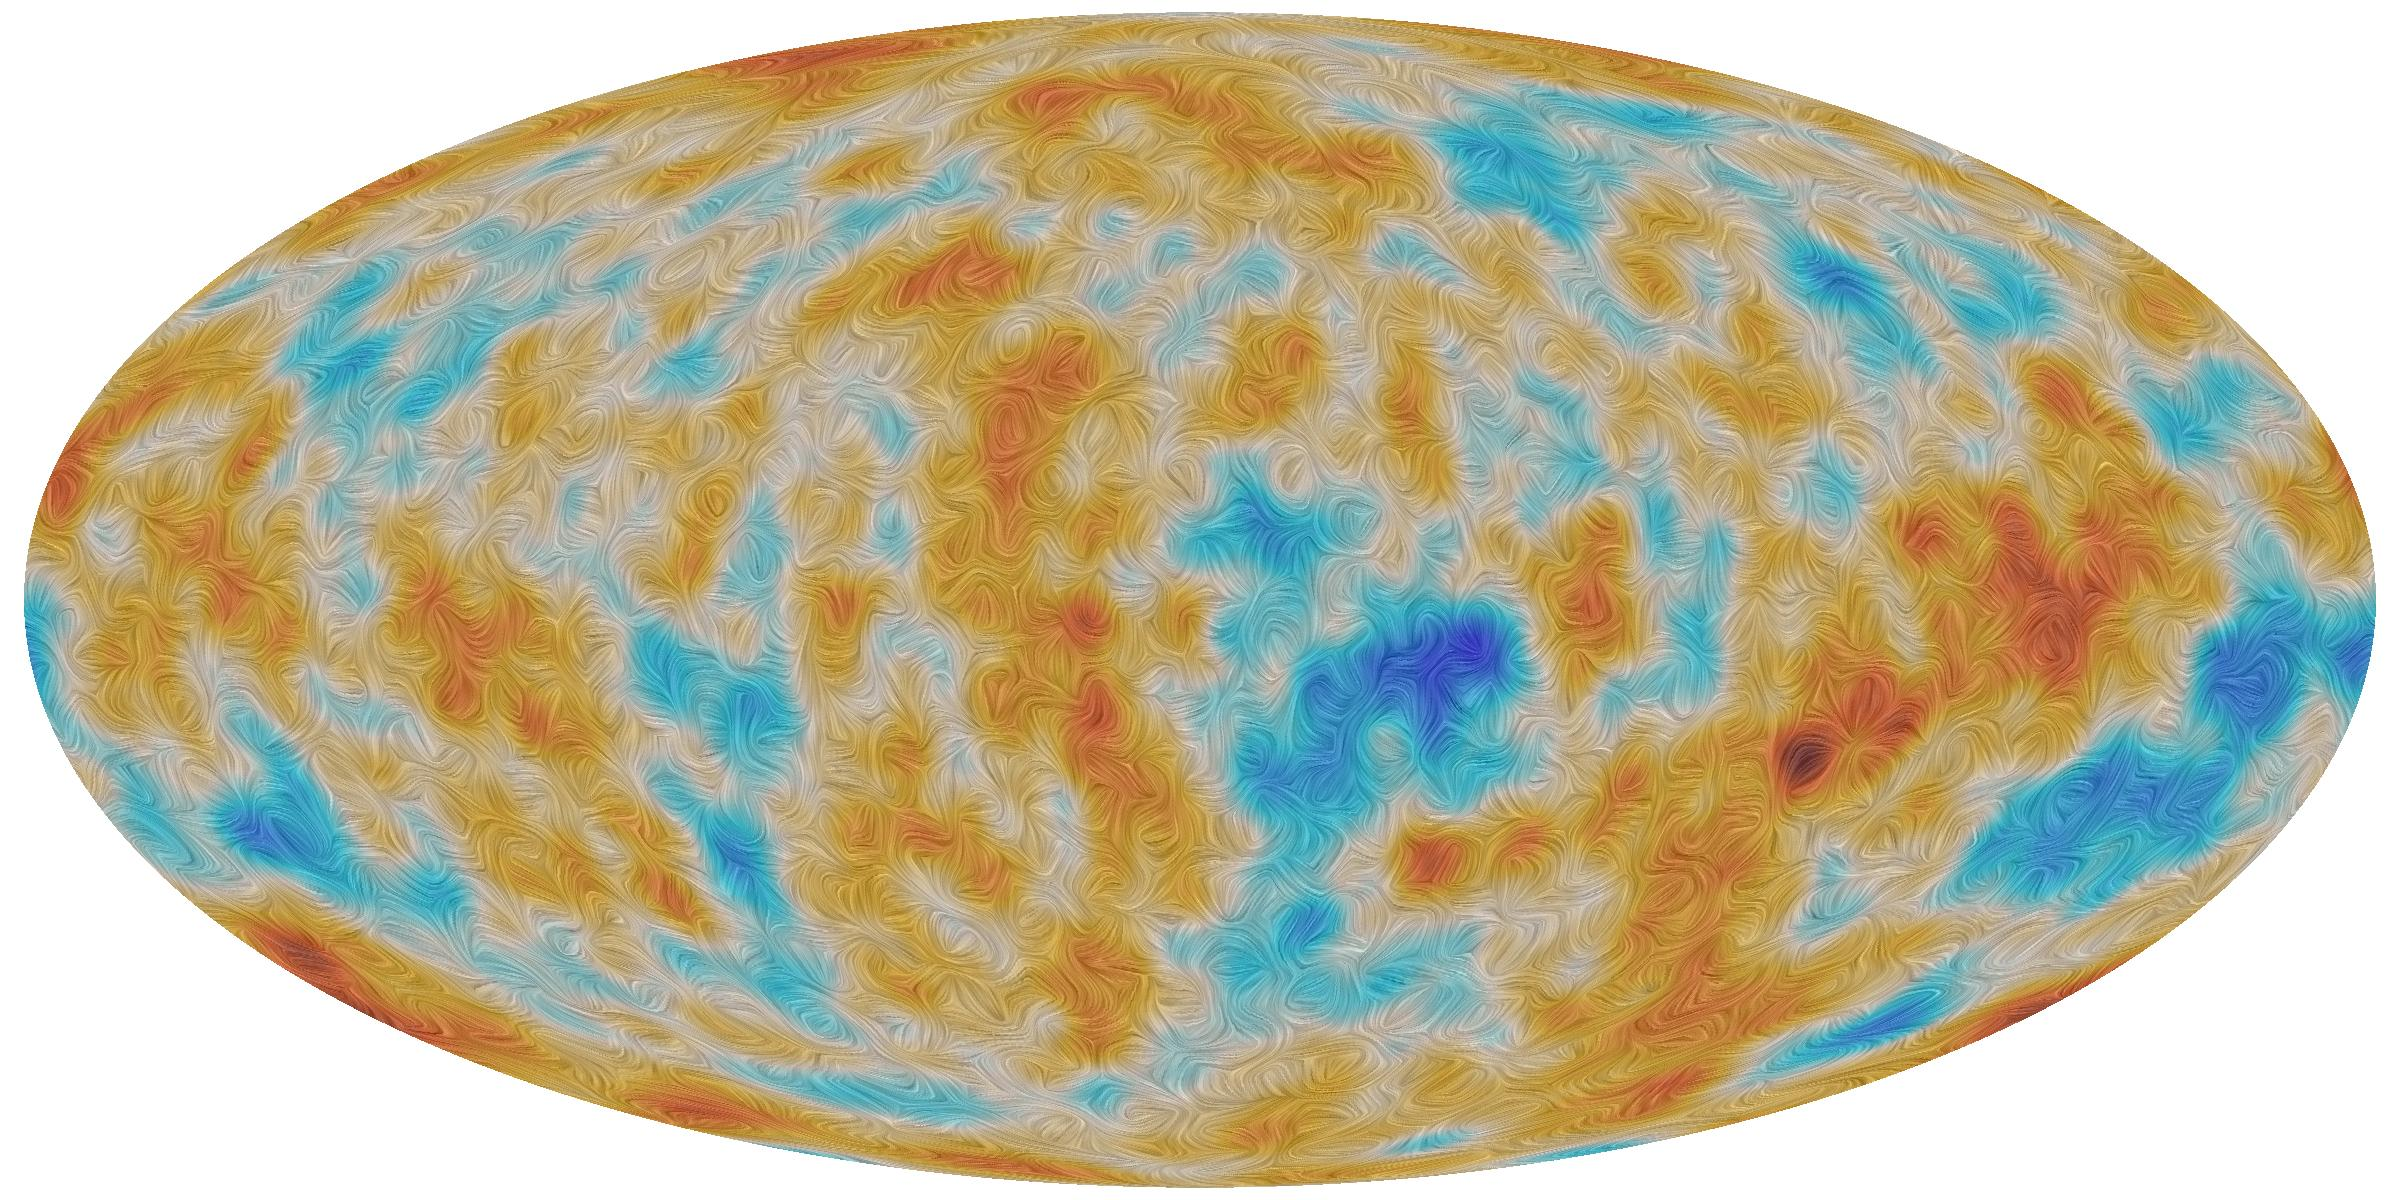
\includegraphics[width=\textwidth]{jpegPIA18916.jpeg}\\
      \textsl{(a)} temperature and polarization
    \end{minipage}
    \begin{minipage}[b]{2in}\noindent%
      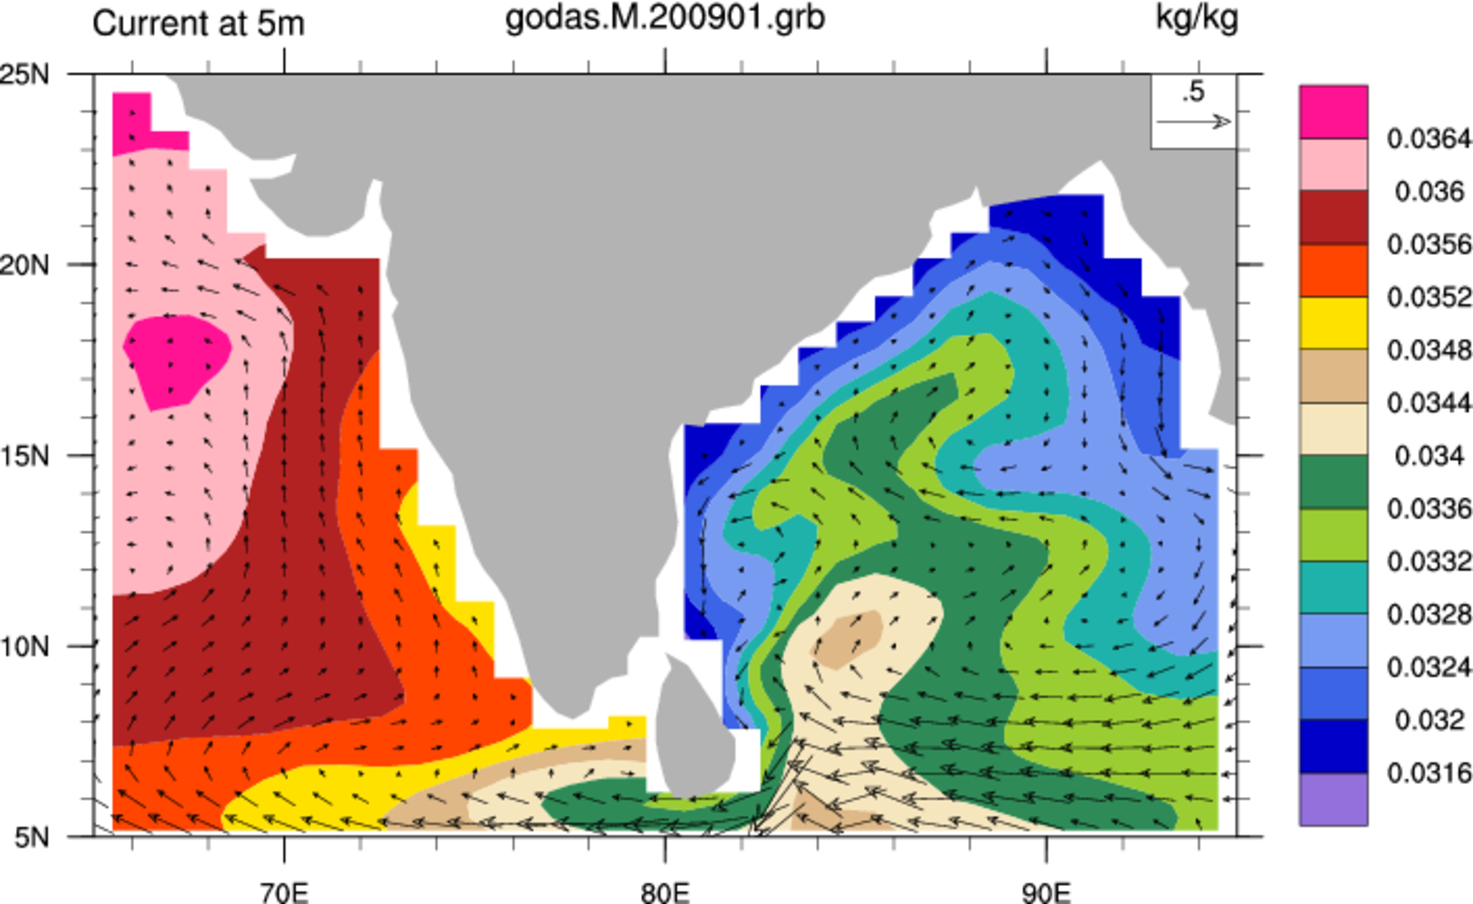
\includegraphics[width=\textwidth]{key_figures_197.pdf}\\
      \textsl{(b)} salinity and current
    \end{minipage}\\[2ex]
    \begin{minipage}[b]{2.5in}\noindent%
      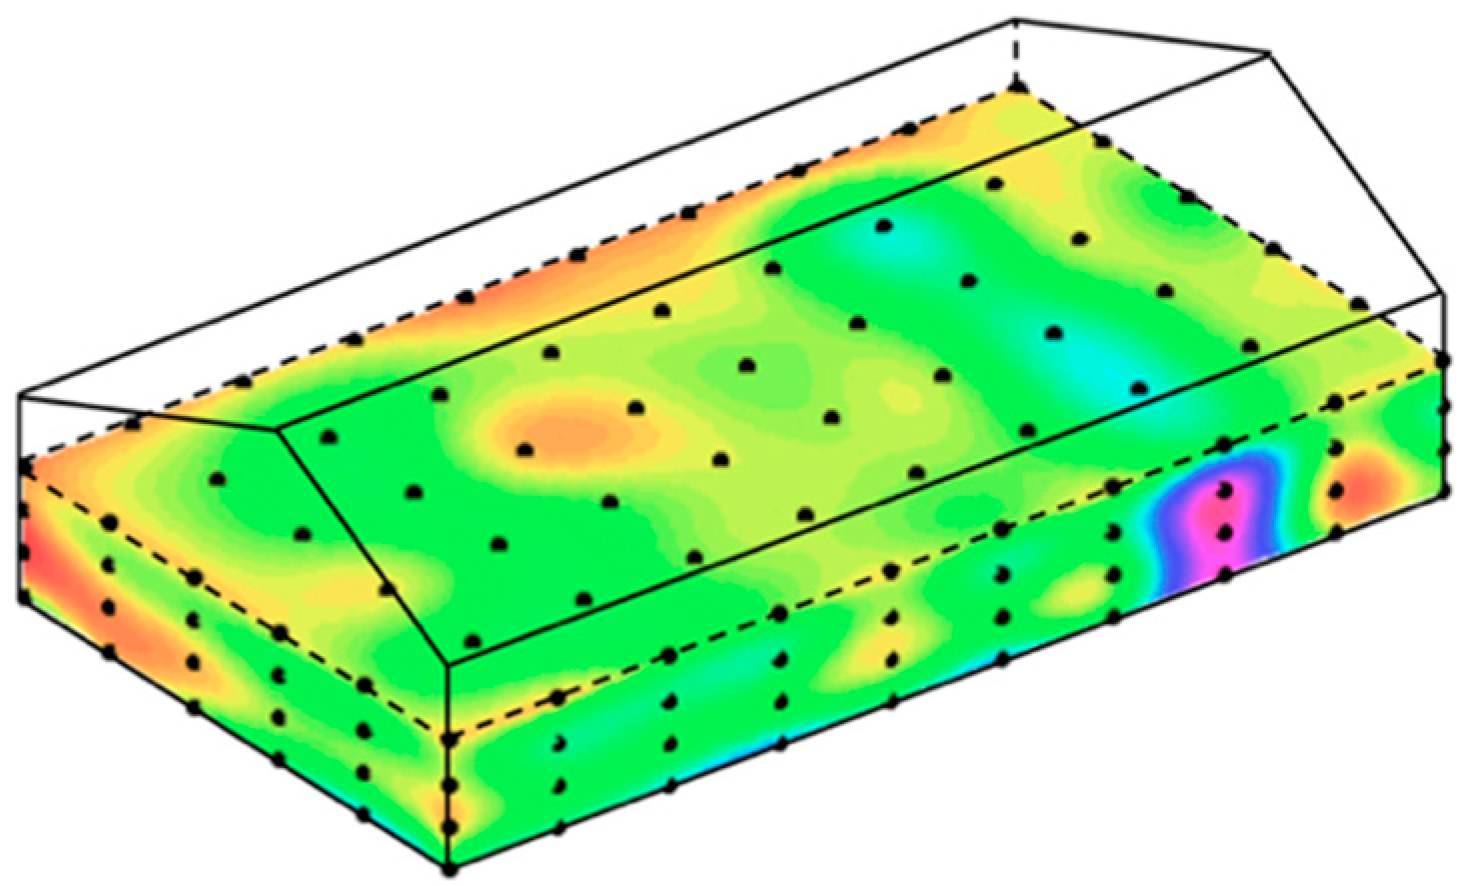
\includegraphics[width=\textwidth]{applsci-09-02108-g001.png}\\
      \textsl{(c)} temperature
    \end{minipage}
    \begin{minipage}[b]{1.8in}\noindent%
      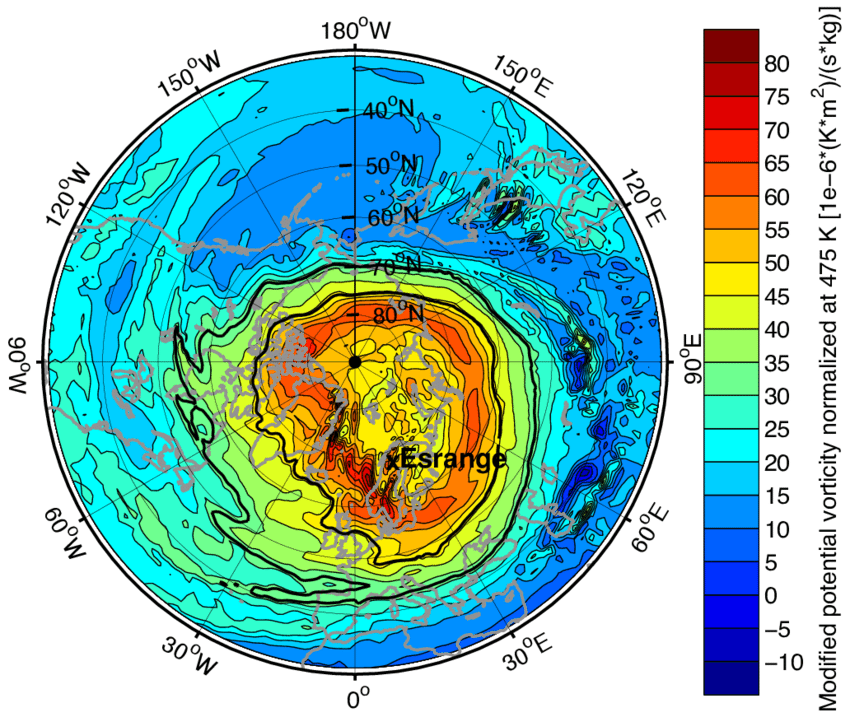
\includegraphics[width=\textwidth]{The-distribution-of-the-modified-potential-vorticity-at-the-850-K-potential-temperature.png}\\
      \textsl{(d)} vorticity
    \end{minipage}\\[2ex]
    \begin{minipage}[b]{1.9in}\noindent%
      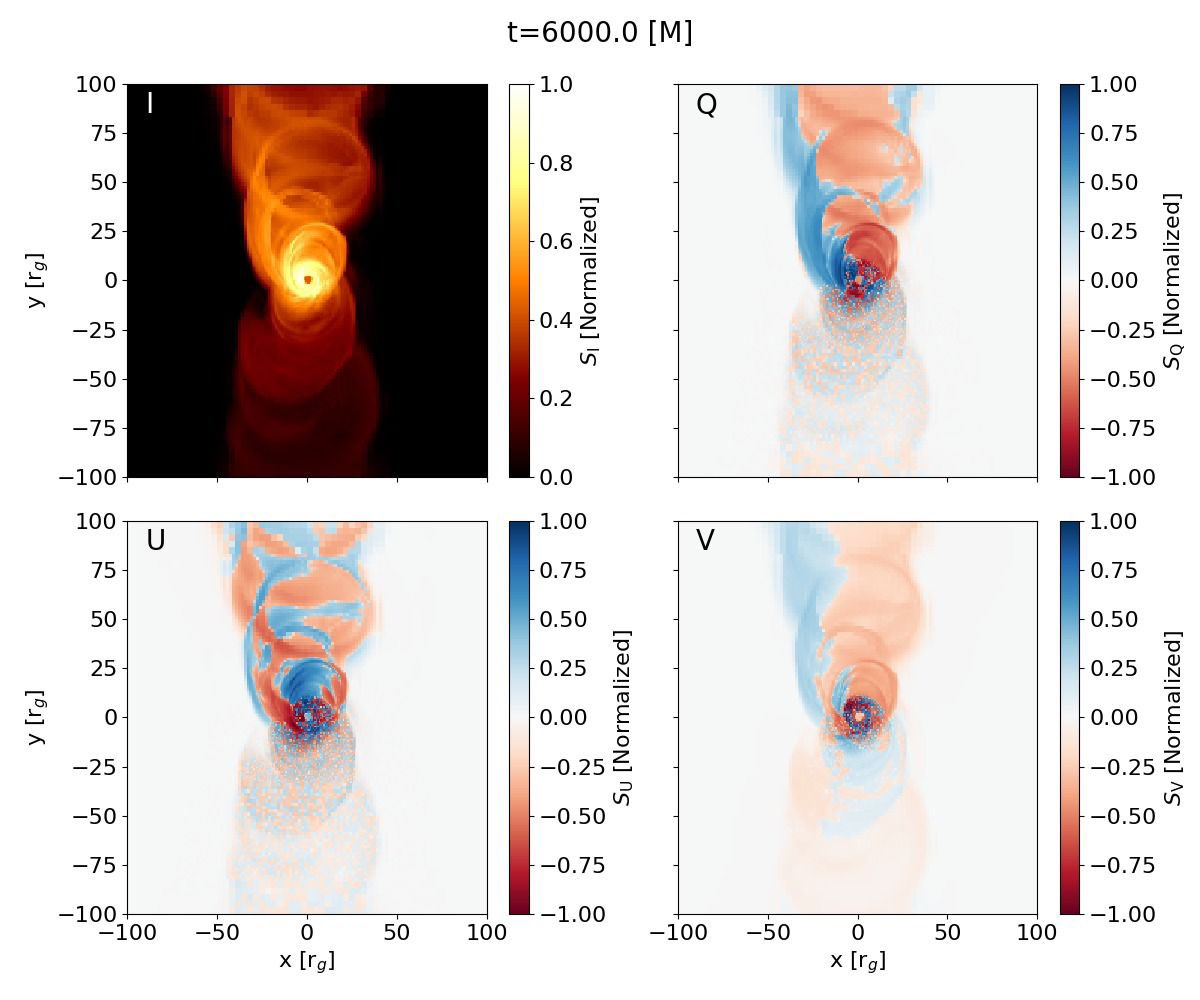
\includegraphics[width=\textwidth]{FbAjqkkWAAANqFc.jpeg}\\
      \textsl{(e)} intensity and polarization
    \end{minipage}
    ~~\begin{minipage}[b]{2.5in}\noindent%
      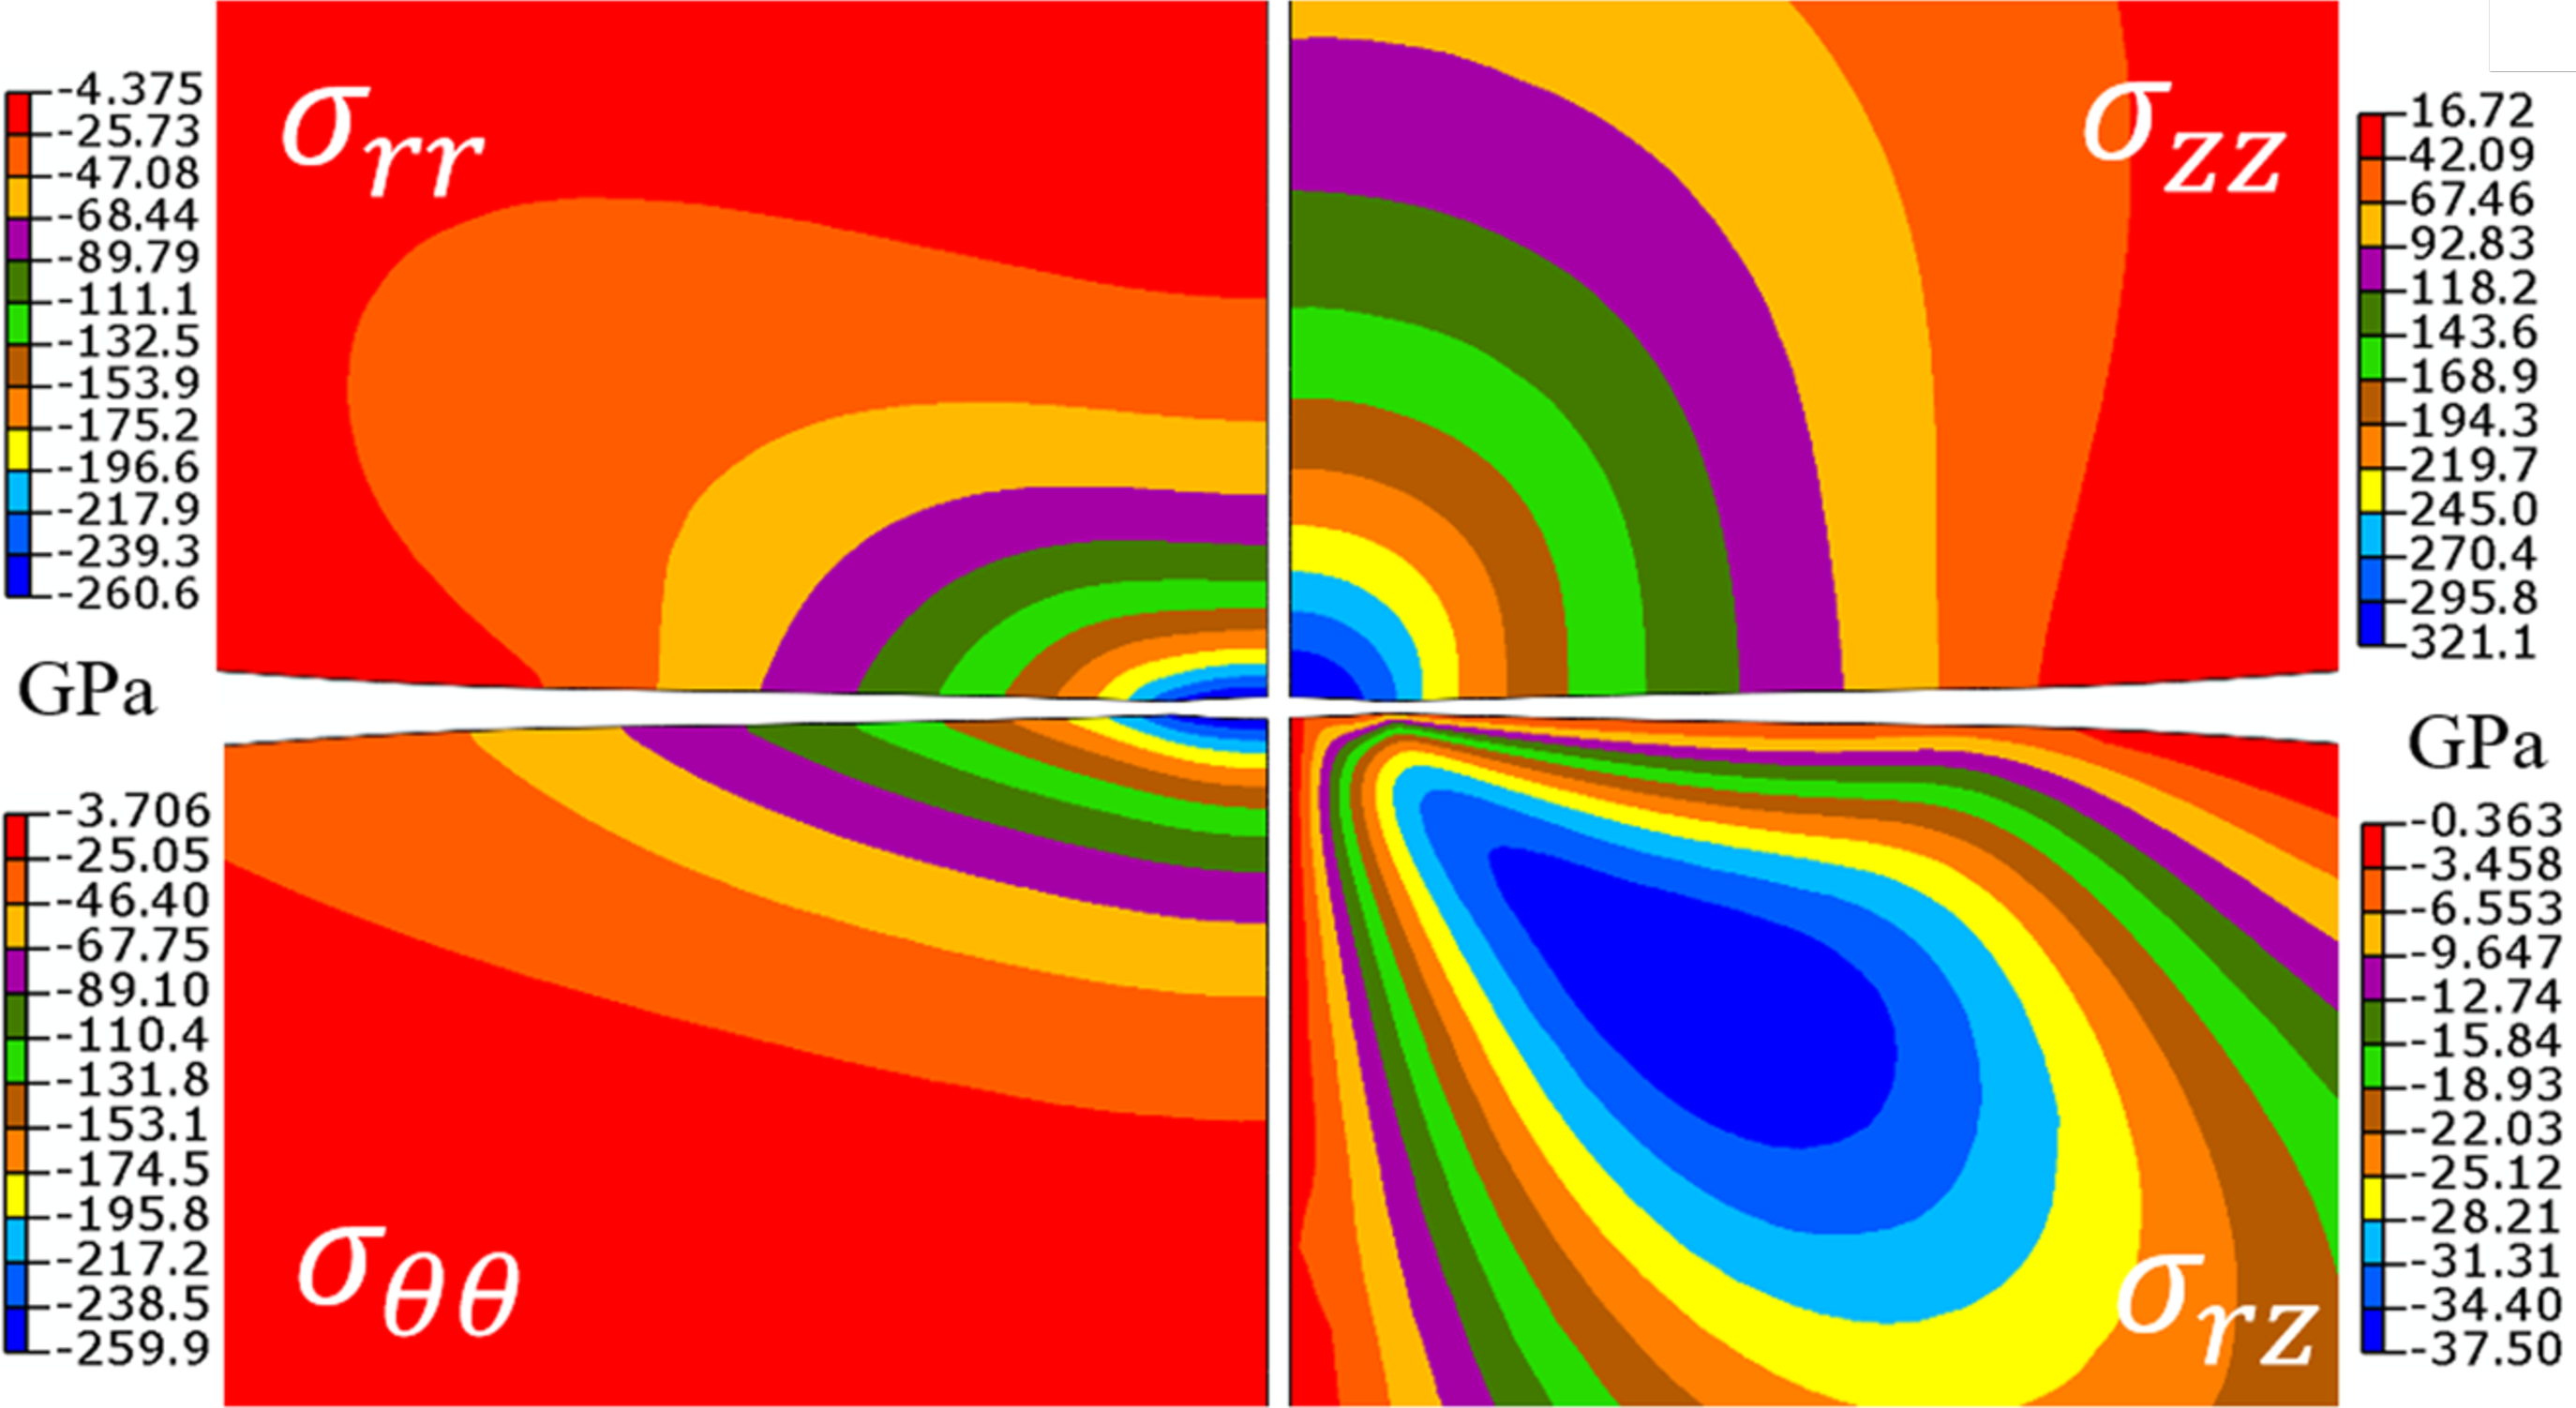
\includegraphics[width=\textwidth]{41524.pdf}\\[1ex]
      \textsl{(f)} stress tensor
    \end{minipage}
  \end{center}
  \caption{Examples of geometric images in the natural sciences.
  \textsl{(a)}~A visualization of a temperature map and a polarization map from the ESA \textsl{Planck} Mission \cite{planck2015}.
  The color map shows a temperature field (a scalar or \tensor{0}{+}) on the sphere, and the whiskers show the principal eigenvector direction of a \tensor{2}{+} field in two dimensions.
  In detail the underlying data are represented on a pixel grid (healpixel \cite{healpix}) on the sky (a 2-sphere).
  \textsl{(b)}~Two-dimensional maps of ocean current (shown with arrows; a vector or \tensor{1}{+} field) and ocean salinity (shown with color; a scalar or \tensor{0}{+} field) at a depth of 5\,m \cite{climatedataguide}.
  \textsl{(c)}~A three-dimensional map of temperature (a scalar or \tensor{0}{+} field) based on sensors distributed throughout the volume of a granary \cite{granary}.
  \textsl{(d)}~A two-dimensional map of potential vorticity (a pseudoscalar or \tensor{0}{-} field) in the Earth's atmosphere, measured for the purposes of predicting storms \cite{potentialvorticity}.
  \textsl{(e)}~Two-dimensional maps on the sky of intensity $I$ and the three independent components $Q, U, V$ of the electromagnetic polarization \tensor{2}{+}, from a simulation of a jet outflow from an accreting black hole [Davelaar et al, in preparation].
  \textsl{(f)}~Components of the three-dimensional stress tensor (a \tensor{2}{+} field) in a diamond anvil cell, which is used to study the behavior of samples at exceedingly high pressures \cite{diamond}.
  \label{fig:examples}}
\end{hoggfigure}

At the present day, the go-to tools for machine learning with images are convolutional neural networks (CNNs; \cite{lecun1989backpropagation}) and their many descendents (for example, CITE).
These methods are designed to work on one- or few-channel images in which the early layers of the network involve image convolutions with learned filters followed by the application of pointwise nonlinearities.
In typical contexts, the channels of multi-channel input images will be something like the red, green, and blue (or cyan, magenta, yellow, and black) channels of a color image; these can be combined arbitrarily in the layers of the CNN.
When these CNN-based tools are applied to lattices of vectors for example, typically the components of the vectors are treated just as channels of the input image (for an example, see CITE) and then everything proceeds as with multi-channel color images.
This is not good! %WILSON: I don't love this. HOGG says: You are the first author. Be bold; edit.

Actually, it \emph{is} good: There are many successful projects that have repurposed CNNs in this way to work on geometric images.
But there are even better choices.
Here we propose a set of tools that generalize the concept of convolution to apply to geometric images such that the outputs of the convolutions are also geometric images, obeying the same geometric transformation rules as the inputs.

The fundamental observation inspiring this work is that when the components of vectors and tensors are acted on with arbitrary functions, the geometric structure of these objects is destroyed.
There are strict rules, dating back to the early days of differential geometry \cite{ricci}, about how geometric objects can be combined to produce new geometric objects, consistent with coordinate freedom and transformation rules (these rules constitute a theme of \cite{mcp}).
In previous work \cite{villar2021scalars, villar2022dimensionless, yao2021simple} we have capitalized on these geometric rules to develop modified machine-learning methods that are restricted to exactly obey group-theoretic equivariances in physics contexts.
Here we use these rules to create a comprehensive set of tools that are universally approximating for functions that take geometric images as input and produce geometric images as output.

We are motivated in this work to help solve problems in the natural sciences, where geometric images abound.
However, we conjecture that these tools are probably very useful even for standard machine-learning image-recognition and image-regression tasks.
After all, even standard images are measurements of intensity (a scalar) at a regular grid of points on a two-dimensional surface.
If the labels we seek are also scalars, it behooves us to obey the rules of geometry.

These rules are roughly as follows:
A $k$-tensor object (tensor of order $k$) in $d$ dimensions has $k$ indices, each of which can take a value from 1 to $d$; that is, the $k$-tensor is an element of $(\mathbb R^d)^{\otimes k}$.
It can be contracted to a $(k-2)$-tensor object by identifying a pair of indices and summing over them.
A $k$-tensor and a $k'$-tensor can be multiplied (outer product) to make a $(k+k')$-tensor object, and then contractions can bring down the order.
$1$-tensor objects are called vectors and $0$-tensor objects are called scalars.
There are also odd-parity versions of all these (pseudovectors, pseudoscalars, and pseudotensors), and parity-changing contractions using the Levi-Civita symbol, so in what follows we will define \tensor{k}{p}s that have $k$ indices and a parity $p\in\{-1,+1\}$, sometimes denoted ``$-$'' and ``$+$'' below.
Two objects can only be added or subtracted if they have the same order $k$ and parity $p$.
These rules define objects that can be given transformation rules under rotation and reflection such that functions made of these operations are coordinate free, or equivariant to any change of coordinate system, including curvilinear coordinate transformations.

The symmetries that suggest these rules are continuous symmetries.
But of course images are usually---and for our purposes---discrete grids of values.
This suggests that in addition to the continuous symmetries respected by the tensor objects in the image pixels there will be discrete symmetries for each geometric image taken as a whole.
We will define these discrete symmetry groups and use them to define a useful kind of group equivariance for functions of geometric images.
This equivariance, it turns out, is very easy to enforce, even for nonlinear functions of geometric images, provided that we compose our nonlinear functions from simple geometric operations, including our geometric generalization of convolution.
When we enforce this equivariance, the convolution filters that appear look very much like the differential operators that appear in discretizations of vector calculus.

\paragraph{Our contribution:}
SOLEDAD: SUMMARY HERE. 
To see a comparison of our work with other methods already studied, see \sectionname~\ref{sec:related}
For a discussion of prior work on group equivariant machine learning, see \sectionname~\ref{sec:related2}.

\section{Non-linear functions of geometric images}

We define the geometric objects and geometric images that we use to generalize classical images in scientific contexts in \sectionname{} \ref{sec:geometric} and \sectionname{} \ref{sec:convolution}, and we define the geometric functions on them in \sectionname{} \ref{sec:nonlinear}.
The main point is that the channels of geometric images---which will be like the components of vectors and tensors---are not independent.
There is an underlying action by the orthogonal group that rules what are the allowed objects and transformations in this space that we describe in \sectionname{}~\ref{sec:equivariant}. 

\subsection{Geometric objects}\label{sec:geometric}

We first fix $d$, the dimension of the space (typically 2 or 3 but it could be arbitrary).
The geometric objects are vectors and tensors. 
The orthogonal group $O(d)$ is the space of isometries of $\mathbb R^d$ that fix the origin. 
%It is represented by matrices $Q\in \mathbb R^{d\times d}$ such that $Q^\top Q = I$. 
It acts on vectors and pseudovectors $v \in \mathbb R^d$ in the following way:
\begin{align} \label{eq.action}
    g\cdot v = \det(M(g))^{\frac{1-p}{2}}\,M(g)\,v
\end{align}
where $g\in O(d)$, $M(g)\in \mathbb R^{d\times d}$ is the standard matrix representation of $g$ (i.e. $M(g)^\top M(g) = I$) and $p\in\{-1,+1\}$ is the parity of $v$.
If $p=+1$ we obtain the standard $O(d)$ action on $\mathbb R^d$ \emph{vectors}.
If $p=-1$ we obtain the $O(d)$ action on what in physics are known as \emph{pseudovectors}.
In this context the objects are defined by the actions that they carry.

\begin{definition}[\tensor{k}{p}s]\label{def.tensors}
We say that $v\in \mathbb R^d$ is a \tensor{1}{p} if $O(d)$ acts on $v$ via the action \eqref{eq.action}. 
If $v_i$ is a \tensor{1}{p_i} then $T:=v_{1}\otimes\ldots \otimes v_k$ is a rank-1 \tensor{k}{p}, where $p=\prod_{i=1}^k p_i$ and the action of $O(d)$ is defined as
\begin{align}
    g\cdot (v_{1}\otimes\ldots \otimes v_k) = (g\cdot v_1)\otimes \ldots \otimes (g\cdot v_k)
\end{align}
Higher rank \tensor{k}{p}s are defined as linear combinations of rank-1 \tensor{k}{p}s where the action of $O(d)$ is extended linearly. The set of \tensor{k}{p}s in $d$ dimensions is denoted $\mathcal{T}_{d,k,p}$.
\end{definition}

\begin{remark}[terminology and notation]
The parity $p$ is a signed bit, either $+1$ for even parity or $-1$ for odd parity.
Note that we call $k$ the \emph{order} of the \tensor{k}{p}, rather than the ``rank'' of the tensor as some other sources do. Using rank for this property is inaccurate because there can be \tensor{2}{+}s of rank 1 (like those we use in Definition~\ref{def.tensors}).
\end{remark}

\begin{remark}[odd-parity objects]
It is possible to replace any odd-parity ($p=-1$) object with an even-parity object with the same physical content by multiplying the odd-parity object by the Levi-Civita tensor (see Definition~\ref{def:levicivita}).
When a \tensor{k}{p} is multiplied (outer product) by a Levi-Civita, the result is a \tensor{(k+d)}{-p}.
Thus, it is possible to work without odd-parity objects at all, in principle.
However, since odd-parity objects are of importance in physics and engineering (see \figurename~\ref{fig:examples}), we retain them.
\end{remark}

In physics the \tensor{1}{+}s (such as velocities) are known as \emph{vectors},
the \tensor{1}{-}s (such as angular momenta) are known as \emph{pseudovectors},
the \tensor{0}{+}s (such as rest masses) are known as \emph{scalars},
the \tensor{0}{-}s (such as surface vorticities) are known as \emph{pseudoscalars},
the \tensor{k}{-}s with $k\geq 2$ are known as \emph{pseudotensors},
and finally the \tensor{k}{+}s with $k\geq 2$ are the things that are commonly known as \emph{tensors}.
In general, any \tensor{k}{p} can be written as a sum of outer products of order-$1$ ($k=1$) tensors (vectors and pseudovectors), where each term in the sum is an outer product of $k$ order-$1$ tensors and the parity $p$ is the product of the parities of the input order-$1$ tensors.

%CONSTANT TENSORS
We consider two special tensors that will be important for the definition of our models, the Kronecker delta and the Levi-Civita.

\begin{definition}[Kronecker delta] The Kronecker delta ($\delta_{ij}$) is a \tensor{2}{+} represented by the identity matrix, namely the object with two indices $ij$ such that it has the value $+1$ when the two indices have the same value ($i=j$), and $0$ otherwise.
\end{definition}

\begin{definition}[Levi-Civita symbol]\label{def:levicivita}
The Levi-Civita symbol in $d\geq 2$ is a \tensor{d}{-} $\epsilon_{i_1,\ldots, i_d}$ such that if the $d$ indices are not repeated and in an even-permutation order the value is $+1$ and if the $d$ indices are not repeated and in an odd-permutation order the value is $-1$, and it has the value $0$ in all other cases.
\end{definition}

\begin{definition}[outer products of tensors]
Given $a \in \mathcal{T}_{d,k,p}$ and $b \in \mathcal{T}_{d,k',p'}$, the outer product, denoted $a\otimes b$, is a tensor in $\mathcal{T}_{d,k+k',p\,p'}$ defined as $[a\otimes b]_{i_1,\ldots,i_{k+k'}} = [a]_{i_1,\ldots,i_k}\,[b]_{i_{k+1},\ldots,i_{k+k'}}$.
\end{definition}

\begin{definition}[contractions and Einstein summation notation]\label{def:contraction}
We use Einstein summation notation where tensor products are written in component form, and repeated indices are summed over.
For example, in this notation, the product of two \tensor{2}{+}s (represented as two $d\times d$ matrices $A$ and $B$) is written as
\begin{equation}
    [A\, B]_{i,j} = [A]_{i,k}\,[B]_{k,j} = \sum_{k=1}^d [A]_{i,k}[B]_{k,j}
\end{equation}
where $[A]_{i,k}$ is the $i,k$ element of matrix $A$, and the sum from 1 to $d$ on repeated index $k$ is implicit in the middle expression.
This notation works for tensor expressions of any order, provided that every index appears either exactly once, so it isn't summed over, or exactly twice, so it is summed over.
\end{definition}

\begin{remark}[lower and upper indices]
In the real Einstein summation notation \cite{einstein}, or Ricci calculus \cite{ricci}, a distinction is made between lower and upper indices, which correspond to covariant and contravariant components.
The pairs of indices that are summed always have one member of the pair an upper index and one member a lower index.
We drop this upper/lower distinction here, because we will work with flat images that implicitly have a trivial metric, such that there is no numerical difference between covariant and contravariant component values for a given object.
That said, there truly is a distinction (for example, if a spatial displacement is a contravariant vector, the gradient of a scalar function with respect to that spatial displacement is a covariant vector), so there might be advantages to reinstating this distinction.
It would complexify method architectures (we discuss these in \secref{sec:architectures}) because the code would have to additionally track the covariance or contravariance of each index of each object.
\end{remark}

One consequence of the above definitions is that 
$T\in (\mathbb R^d)^{\otimes k}$ is a \tensor{k}{p} if and only if, in summation notation,
\begin{align}
    [g\cdot T]_{i_1,\ldots, i_k} = \det(M(g))^{\frac{1-p}{2}}\,[T]_{j_1,\ldots,j_k}\,[M(g)]_{i_1,j_1}\cdots[M(g)]_{i_k,j_k}
\end{align} for all $g\in O(d)$, where $[T]_{i_1, \ldots ,i_k} \in \mathbb R$ is a component of $T$, $[M(g)]_{i,j}\in\mathbb R$ is the $i,j$ element of the matrix representation of $g$, and all the $i_m$ and $j_m$ are indices in the range $1,\ldots,d$.
For example, a \tensor{2}{+} is defined by its transformation property
$[g\cdot T]_{i,j} = [T]_{k,\ell}\,[M(g)]_{k,i}\,[M(g)]_{\ell,j}$,
which, in normal matrix notation, is written as
$g\cdot T = M(g)\,T\,M(g)^\top$.

We can combine multiplication with Kronecker and Levi-Civita symbols with contractions to define relevant operations. For example the \tensor{2}{+} formed by the outer product of \tensor{1}{+}s $a$ and $b$ can be contracted with the Kronecker delta to give the standard dot product $a^\top b = [a]_i\,[b]_j\,\delta_{ij}$, which is a \tensor{1}{+} or scalar.
For another example, the same \tensor{2}{+} can (in $d=3$ dimensions) be contracted with the Levi-Civita symbol to give the standard cross product
$[a\times b]_k = [a]_i\,[b]_j\,\epsilon_{ijk}$, which is a \tensor{1}{-} or pseudovector.

\begin{definition}[permutations of tensor indices]
Given $a \in \mathcal{T}_{d,k,p}$ and permutation sequence $\sigma\in S_k$, the permutation of $a$ by $\sigma$, denoted $a^\sigma$, is:
\begin{equation}
    [a^\sigma]_{i_1, \ldots, i_k} := [a]_{\sigma^{-1}(i_1), \ldots, \sigma^{-1}(i_k)}
\end{equation}
\end{definition}

\begin{comment}
(WILSON PONDERS: I think I might just cut this below, I understand that physicists think about tensors in this way, but if we aren't using it I don't think it adds much.) There is an alternative definition of \tensor{k}{p}s in terms of geometric functions (see, for example, \cite{mcp} chapter 1):
A \tensor{k}{+} can be thought of as representing a multilinear function of $k$ vectors (\tensor{1}{+}s) that produces a scalar (\tensor{0}{+}) output.
For example, if $A$ is a \tensor{4}{+}, and $u,v,w,x$ are vectors (\tensor{1}{+}s) then (in summation notation)
\begin{equation}
    \rho = [A]_{ijk\ell}\,[u]_i\,[v]_j\,[w]_k\,[x]_\ell
\end{equation}
is a scalar (\tensor{0}{+}).
\tensor{k}{-}s can be similarly defined in terms of input vectors and an output pseudoscalar.
\end{comment}

\subsection{Geometric images and convolutions}\label{sec:convolution}

We consider an image $A$ in with $N$ equally spaced pixels in each dimension ($N^d$ pixels total). Each pixel contains a \tensor{k}{p} where $k$ and $p$ are the same for each pixel. Sometimes we will consider the image to be in a $d$-torus. 
Let $\mathcal T_{d,k,p}$ the set of \tensor{k}{p}s in $\mathbb R^d$. We define the geometric images as follows.

\begin{definition}[geometric image]
A geometric image is a function $A:[N]^d \to \mathcal T_{d,k,p}$, where $[N]=\{0,1,\ldots, N-1\}$. The set of geometric images is denoted $\mathcal{A}_{N,d,k,p}$. We will also consider \tensor{k}{p} images on the $d$-torus, where $[N]^d$ is given the algebraic structure of $(\mathbb Z / N\mathbb Z)^d$.
\end{definition}

In this \sectionname{} we generalize the notion of convolution to take geometric images as inputs and return geometric images as outputs.
The idea is that a geometric image of \tensor{k}{p}s is convolved with a geometric filter of \tensor{k'}{p}s to produce a geometric image that contains \tensor{(k+k')}{p\,p'}s, where each pixel is a sum of outer products. These outer products can be contracted down to lower-order tensors using contractions (Definition~\ref{def:contraction}). Note that the sidelength $N$ of the geometric image is typically much larger than the sidelength $M$ of the geometric filter.

\begin{definition}[geometric convolution]\label{def:convolution}
Let $A \in \mathcal{A}_{N,d,k,p}$ on the $d$-torus, and let $C \in \mathcal{A}_{M,d,k',p'}$ where $M=2m+1\leq N$.
The geometric convolution $A\ast C$ is a \tensor{(k+k')}{p\,p'} image such that
\begin{equation}
    (A\ast C)(\bar\imath) = \sum_{\bar a\in[-m, m]^d} A(\bar\imath - \bar a)\otimes C(\bar a) ~,
\end{equation}
where $\bar\imath - \bar a$ is the translation of $\bar\imath$ by $\bar a$ on the $d$-torus pixel grid $(\mathbb Z / N\mathbb Z)^d$.
\end{definition}
This definition is on the torus. To define the convolution in $[N]^d$ instead of the torus, we can pad the image out with zero tensors of the corresponding order and parity. 

In addition to contractions and index permutations that act pixel-wise in geometric images, it is possible to change the image size.
If $N$ is divisible by integer $f>1$, a geometric image of side length $N$ can be reduced in size to a geometric image of side length $N/f$ by the equivalent of convolution with a trivial $f\times f$ scalar filter (geometric filter of \tensor{0}{+}s) operating with a stride of $f$.
Similarly a geometric image of side length $N$ can be expanded in size to a side length $f\,N$ by application of an interpolation operator with stride $1/f$.

\subsection{Higher-order functions of geometric images}\label{sec:nonlinear}

The convolution, contraction, index-permutation, and pooling operators above effectively span a large class of linear functions from geometric images to geometric images. Non-linear functions can be constructed as polynomials, or sums of products of linear function outputs.
Products here will be outer products, possibly followed by further geometric convolutions and contractions.

\begin{definition}[outer products of images]
Given $A \in \mathcal{A}_{N,d,k,p}$ and $B \in \mathcal{A}_{N,d,k',p'}$, the outer product $A\otimes B \in \mathcal{A}_{N,d,k+k',p\,p'}$ is defined as
\begin{equation}
    (A\otimes B)(\bar\imath) = A(\bar\imath)\otimes B(\bar\imath) ~.
\end{equation}
for each pixel $\,\bar\imath$. That is, the outer products of geometric images are performed pixel-wise.
\end{definition}

\begin{definition}[sums of images]
Given $A,B \in \mathcal{A}_{N,d,k,p}$, the sum $A+B \in \mathcal{A}_{N,d,k,p}$ is defined as
\begin{equation}
    (A+B)(\bar\imath) = A(\bar\imath)+B(\bar\imath) ~.
\end{equation}
for pixel $\,\bar\imath$. That is, the sums of geometric images are performed pixel-wise.
\end{definition}

HOGG IS CONFUSED: HOW ARE WE MAKING $N'\ne N$ IN THE BELOW?

Now to construct all degree-2 monomials that produce a \tensor{k'}{p'} image of side length $N'$ output from a \tensor{k}{p} image of side length $N$ input, here are the rules:
\begin{enumerate}
    \item By the rules in \secref{sec:convolution}, construct any linear function that takes the input geometric image and outputs a geometric image of any order $k''$ and any parity $p''$ and any side length $N''$.
    \item By the rules in \secref{sec:convolution}, construct any other linear function that takes the input geometric image and outputs a geometric image of any order and any parity.
    There is no need for this second output image to be the same order or parity as the first, but it does have to have the same side length.
    \item Outer product these two images.
    \item By the rules in \secref{sec:convolution}, construct any linear function that takes this image outer product as input and produces a \tensor{k'}{p'} image of side length $N'$ as output.
\end{enumerate}

We conjecture that these rules will generate all possible second-degree monomial functions of the input image as long as the filter size is sufficiently large (BEN, is this correct?). A polynomial function of degree 2 can be constructed by linear combinations of these second-degree monomial functions along with all the linear functions that also produce \tensor{k'}{p'} images of side length $N'$ (plus perhaps constant images).
Higher-degree monomials and polynomials can be made out of products of lower-degree monomials, by generalization of the above.

The geometric convolutions of \secref{sec:convolution} are local linear operators that take as input geometric images, and produce as output geometric images.
They are local in the sense that, at every pixel $\bar\imath$ of the output image $(A\ast C)$, the convolution only makes use of the pixels of $A$ within a small neighborhood of of $\bar\imath$.
Because tensors can be multiplied together using the outer product, and contracted according to the tensor contractions defined in \secref{sec:convolution}, it is possible, by multiplication, to construct a family of \emph{nonlinear} local geometric operators that take as input geometric images and produce as output geometric images.
This family of nonlinear local operators will be equivariant to the group $G_{N,d}$ when the linear local operators of which they are composed are equivariant.

\section{Equivariant functions of geometric images}\label{sec:equivariant}


Convolutional filters are widely used in machine learning for scalar images. The fundamental property of these operators are that they are translation equivariant, and that every translation equivariant linear function can be expressed as a convolution with a fixed filter (as long as the filter can be set to be as large as the image). The same property holds for geometry images.

\begin{definition}[Translation of \tensor{k}{p} images and translation equivariance] Given a \tensor{k}{p} image $A$ on the $d$-torus, and a translation $\tau \in (\mathbf{Z}/N \mathbf{Z})^d$, the action $L_\tau A$ produces a \tensor{k}{p} image on the $d$-torus such that
\begin{equation}
    (L_\tau A)(\bar \imath) = A(\bar \imath-\tau)
\end{equation}
where $\bar\imath - \tau $ is the translation of $\bar\imath$ by $\tau$ on the $d$-torus pixel grid $(\mathbb Z / N\mathbb Z)^d$.
A function $f:\mathcal A_{N,d,k,p}\to A_{N,d, k'', p''}$ is translation equivariant if $f(L_\tau A) = L_\tau f(A)$ for all $A\in \mathcal A_{N,d,k,p}$ and $ \tau \in (\mathbf{Z}/N \mathbf{Z})^d$.
\end{definition}
It follows directly from the Definition \ref{def:convolution} that the convolution with a geometric filter \tensor{k'}{p'} filter is translation equivariant:
\begin{equation*}
    (L_\tau A\ast C)(\bar\imath) = \sum_{\bar a\in[-m, m]^d} A((\bar\imath-\tau) - \bar a)\otimes C(\bar a)= L_\tau (A\ast C)(\bar \imath).
\end{equation*}

\begin{proposition}
A function $f:\mathcal A_{N,d,k,p}\to A_{N,d, k'', p''}$ is a linear translation equivariant linear function if and only if it is the convolution with a geometric filter \tensor{k'}{p'} filter $C$ with possibly sidelength $N$, where $k+k'=k''$ and $p\,p'=p''$.
\end{proposition}
\begin{proof}
TO DO. Also say this is a particular case of bigger theoretical results, e.g. cite results by T. Cohen and R. Kondor. \textcolor{blue}{Is this Proposition 1 true? Consider the case $N=1$, $A_{1,d,k,p}\cong T_{d,k,p} \cong \mathbf{R}^{d^k}$. In this case, all functions $f:\mathcal A_{1,d,k,p}\to A_{1,d, k'', p''}$ are translation equivariant. But it is not true that all linear translation equivariant linear functions are the convolution with a geometric filter: e.g. $d=2, k=1, k''=2$, then $\mathcal A_{1,2,1,p}\cong \mathbf{R}^2$ and $\mathcal A_{1,2,2,p}\cong \mathbf{R}^4$, the linear function
$(x_1,x_2)\mapsto (0,0,0, \lambda x_1+\beta x_2)$ is not a convolution with a geometric filter, since a \tensor{1}{p} image is $C=(c_1, c_2)$ and the convolution $(x_1,x_2)\mapsto (x_1,x_2)\otimes(c_1,c_2)=(c_1x_1, c_1x_2, c_2x_1, c_2x_2)$ }
\end{proof}

In addition to translation symmetries, we want to consider other natural symmetries occurring in the application domains where vectors and tensors arise. Ideally we would like to apply continuous rotations to the images, but their discretized nature makes it challenging. Recent work has proposed an approach to approximate continuous symmetries \cite{} that require interpolating and cropping the images. Here, for simplicity we focus on discrete rotations as in \cite{}, and we extend the group action to the geometric objects in the images.

\begin{definition}[Group $B_d$ of symmetries of a $d$-hypercube]
We denote by $B_d$ the group of Euclidean symmetries of the $d$-dimensional hypercube.
\end{definition}

The group $B_d$ is often called the {\em hyperoctahedral group} since the $d$-dimensional hyperoctahedron (also known as the cross-polytope) is dual to the hypercube, so they have the same group of symmetries. The notation $B_d$ is standard nomenclature coming from the classification theorem for finite irreducible reflection groups \cite{humphreys1990reflection}.

%BBS: I made minor edits. In representation theory and algebraic combinatorics it is called the hyperoctahedral group. Imo, ``rotation and reflection symmetries" was a misnomer, this just captures the symmetries with fixed point sets of codimension 1 and 2. When $d\geq 4$, there are others. (I'm being a nomenclature partisan in that some people do use ``rotation" to mean any element of $SO(d)$, whereas I only use it to mean a literal rotation in a plane (fixing the plane's complement). But even with the more liberal meaning of rotation, ``rotations and reflections" still does not include the elements with fixed point sets of odd codimension >1, since these are not in $SO(d)$.) I changed it to Euclidean symmetries.

Notes about the group $B_d$: It has $2^d\cdot d!$ elements (so in $d=2$ there are $8$ elements, in $d=3$ there are $48$, and in $d=4$ there are $384$). Because the groups $B_d$ are subgroups of $O(d)$, all determinants of the matrix representations of the group elements are either $+1$ or $-1$, and the matrix representation $M(g^{-1})$ of the inverse $g^{-1}$ of group element $g$ is the transpose of the matrix representation $M(g)$ of group element $g$.

Note that because $B_d$ is a subgroup of $O(d)$, the action of $B_d$ on \tensor{k}{p}s is the restriction of the action in Definition \ref{def.tensors} to the subgroup.

\begin{definition}[Action of $B_d$ on \tensor{k}{p} images]
Given a \tensor{k}{p} image $A$ on the $d$-torus, and a group element $g\in B_d$, the action $g\cdot A$ produces a \tensor{k}{p} image on the $d$-torus such that
\begin{equation}
    (g\cdot A)(\bar\imath) = g\cdot A({g^{-1}\cdot \bar\imath}) ~.
\end{equation}
SOmeThiNg about how $g^{-1}\cdot\bar\imath$ works here, possibly preceded or followed by proofs. Because of what follows, this has to be defined BOTH for the $N^d$ boxels in the $d$-torus and on the $(2\,m+1)^d$ boxels of the filter (image patch).
\end{definition}

It might be a bit surprising that the group element $g^{-1}$ appears in the definition of the action of the group on images.
One way to think about it is that the pixels in the output (rotated, say) image are ``looked up'' or ``read out'' from the pixels in the original (unrotated) image.
The pixel locations in the original image are found by going back, or inverting the transformation.

HOGG: Make a table and a figure showing all the group operators in $B_d$ with $d=2$.

\begin{definition}[The group $G_{N,d}$, and its action on \tensor{k}{p} images]\label{def:GdN}
THIS NEEDS TO BE WRITTEN: $G_{N,d}$ is the group generated by the elements of $B_d$ and the discrete translations on the $N^d$-pixel lattice on the $d$-torus.
\end{definition}

BBS: Somewhere here we should mention the canonical map $G_{N,d} \rightarrow B_d$ obtained by quotienting out by the translations. (This is used in the Hilbert series computation below.) Should I write this part?

HOGG: Comment on the fact that $G_{N,d}$ is a subgroup of the Euclidean group, but that we care about the Euclidean group because we are imagining that the discrete images are images of a continuous world!!

\begin{definition}[Equivariant convolution]\label{def:GNd equivariant}
We say that a convolution filter $C$ produces convolutions that are equivariant with respect to the group $G_{N,d}$ if for any \tensor{k}{p} image $A$ on the $d$-torus, and any group element $g\in G_{N,d}$, we have
\begin{equation}
    g\cdot (A\ast C) = (g\cdot A)\ast C ~,
\end{equation}
where the group actions are defined above.
\end{definition}

The intuition here is that the filter $C$ represents some physical law, and the image $A$ represents the initial conditions or state of the physical system on which the law is acting.
The physical law (represented by $C$) is invariant to translations, rotations, and parity, while the \emph{output} of the physical law (represented by $A\ast C$) is \emph{equivariant} to translations, rotations, and parity acting on the state $A$.

The following theorem generalizes the Cohen and Welling paper:

\begin{theorem}
A \tensor{k'}{p'} convolution filter $C$ produces convolutions that are equivariant with respect to the big group $G_{N,d}$ if $C$ is invariant under the small group $B_d$.
\end{theorem}

\begin{proof}
By Definition \ref{} we have
\begin{eqnarray}
(g\cdot (A* C) )(\bar \imath) &=& g\cdot( (A*C)(g^{-1} \cdot \bar \imath)) \\
&=& g \cdot \left (\sum_{a\in [-m,m]^d} A(g^{-1}\cdot \bar \imath - a) \otimes C(a)\right)\\
&=& \sum_{a\in [-m,m]^d} g \cdot A(g^{-1} \cdot \bar \imath -a ) \otimes g \cdot C(a).
\end{eqnarray}
By Definition \ref{} we have
\begin{eqnarray}
((g\cdot A)* C) (\bar \imath) &=& \sum_{a\in [-m,m]^d} g\cdot A(g^{-1} \cdot (\bar \imath - a) ) C(a) \\
&=& \sum_{a'\in [-m,m]^d} g \cdot A(g^{-1}\cdot \bar \imath -a') \otimes C(g\cdot a'),
\end{eqnarray}
where $a'=g\cdot a$. Therefore the convolution is equivariant if $g\cdot C(g^{-1} \cdot a') = C(a')$ for all $g\in B_d$ and all $a' \in [-m,m]^d$. 
\end{proof}

In practice, a complete set of invariant \tensor{k'}{p'} filters (filters $C$ such that $g\cdot C(g^{-1} \cdot a') = C(a')$) can be found by group averaging.
This works by, for each setting of order $k'$ and parity $p'$, building a collection of linearly independent \tensor{k'}{p'} filters (randomly or systematically), and then building, for each of these linearly independent filters $C$, a group-averaged filter $\bar{C}$ by
\begin{equation}
    \bar{C}(a') = \frac{1}{|B_d|}\,\sum_{g\in B_d} g\cdot C(g^{-1}\cdot a') ~,
\end{equation}
where $|B_d|$ is the number of group elements (8 for $d=2$ and 27 for $d=3$).
In detail we took a systematic (not random) approach that, for each setting of $(k',p')$, initialized the averaging with a set of independent \tensor{k'}{p'} convolution filters that span the space of all possible geometric convolution filters at side length $M$ ($M=2\,m+1$) and dimension $d$.
There are $M^d\,d^{k'}$ independent filters in this initial set.
The averaged filters are then reduced to an ``eigen-set'' of orthogonal, non-zero filters by the singular-value decomposition.
The singular-value decomposition reduces the number of filters dramatically.
The outputs of the singular-value decomposition can be normalized however seems appropriate.
In detail we normalized to get unit tensor norms in the non-zero pixels.
The results of these operations are shown for $d=2$ and $m\in[1, 2]$ in \figref{fig:filters23} and \figref{fig:filters25}.
HOGG: Give a table saying how many filters there are for each tuple of $(d,m,k',p')$.
HOGG: Perhaps remind the reader that the code is available.
\begin{hoggfigure}
  \begin{center}
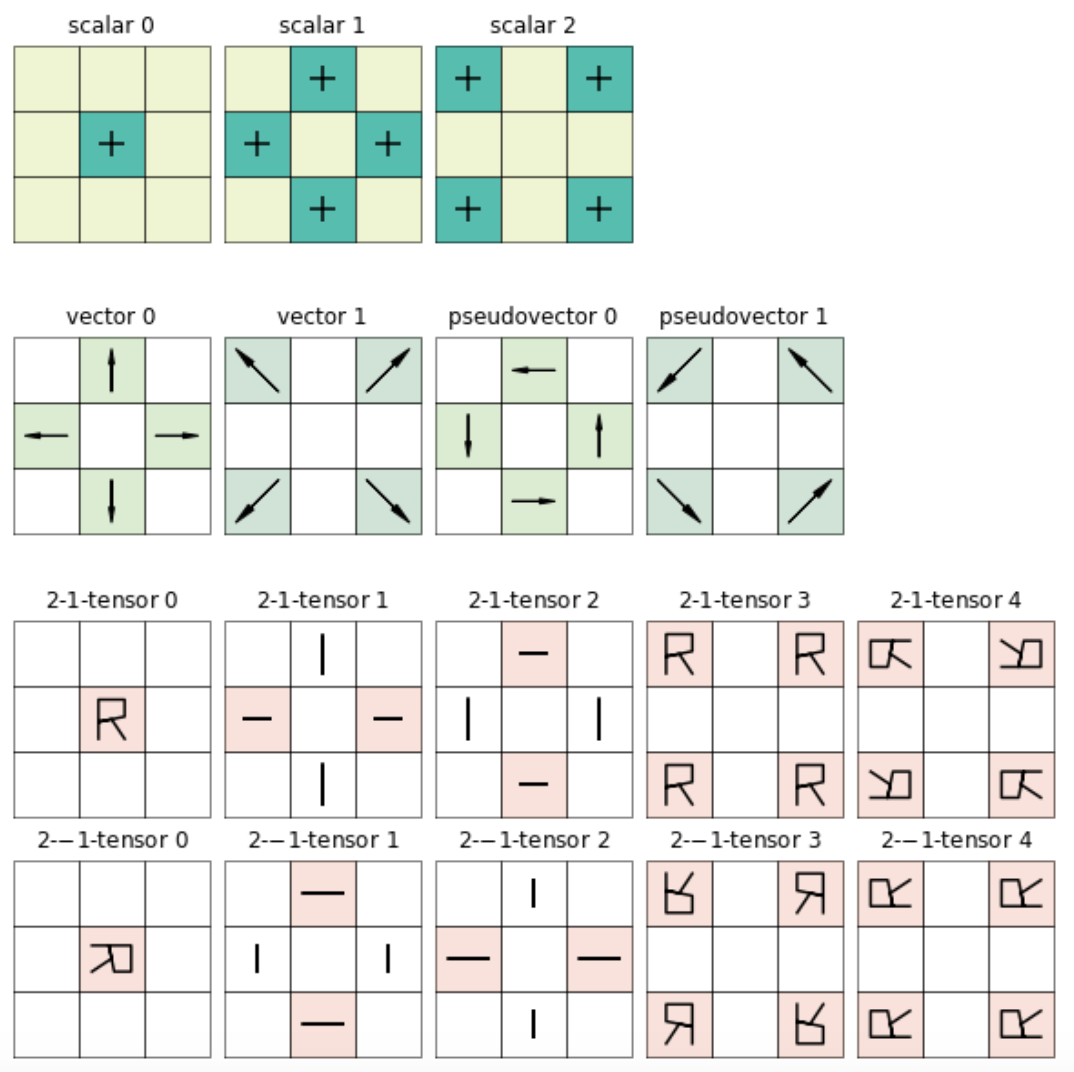
\includegraphics[width=\textwidth]{pics/invariant_filters.png}
  \end{center}
\caption{All the filters for $d=2$, $m=1$ ($M=3$), $k'\in [0,1,2]$.
Notes: Scalars and pseudo-scalars are shown with signed colors; where there is no symbol in the box the value is zero. The \tensor{2}{p'} filters are shown via the action of the tensor on an image of a letter ``R''; the transformation properties of the \tensor{2}{p'} filters are such that these filters may not look obviously invariant to rotations, but they are, gosh darn it.
There are no invariant pseudoscalar (\tensor{0}{-}) filters available at $(d,m) = (2,1)$.
Note that the \tensor{2}{+} 0 and \tensor{2}{+} 3 filters are duplicates of the \tensor{0}{+} 0 and \tensor{0}{+} 2 filters respectively after they are multiplied by the identity tensor. Additionally, if we add \tensor{2}{+} 1 and \tensor{2}{+} 2 it is the same as \tensor{0}{+} 1 multiplied by the identity tensor. We don't show the \tensor{k'}{p'} filters at $k'>2$ because visualizing them is difficult, even the $k'=2$ case is potentially misleading.
Note that the vector (\tensor{1}{+}) filters look like pure divergence and the pseudovector (\tensor{1}{-}) filters look like pure curl.\label{fig:filters23}}
\end{hoggfigure}
\begin{hoggfigure}
  \begin{center}
    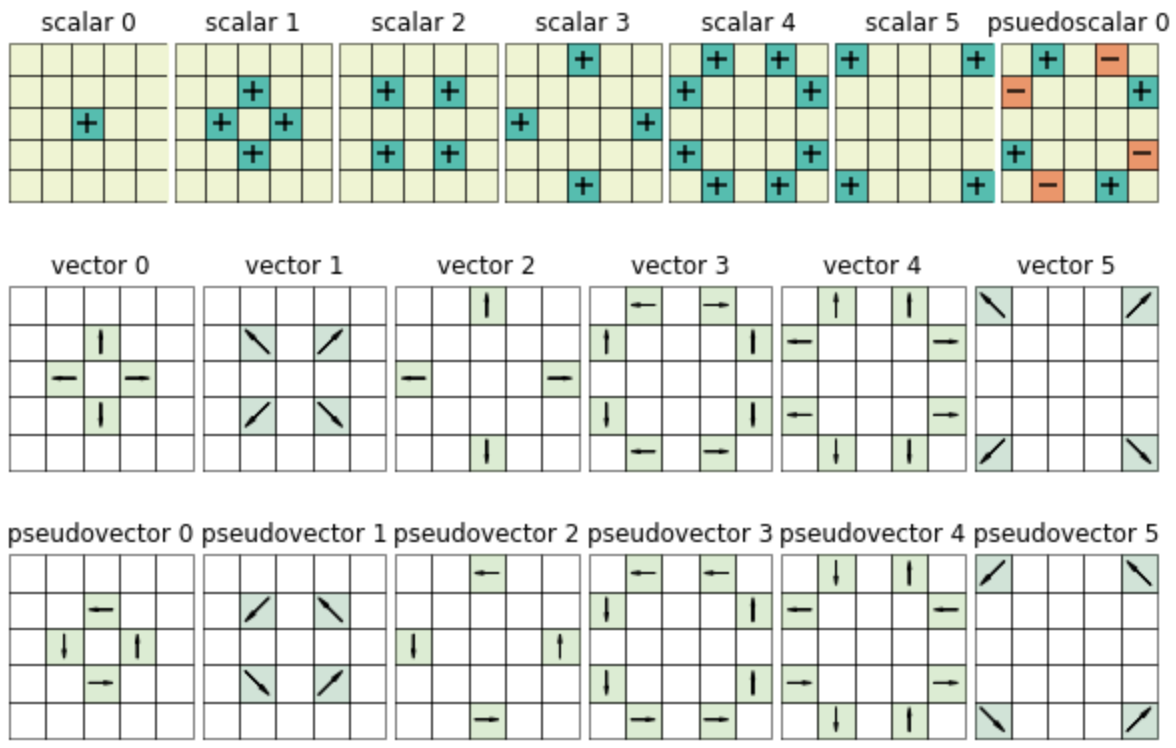
\includegraphics[width=\textwidth]{pics/filters_m5.png}
  \end{center}
\caption{All the filters for $d=2$, $m=2$ ($M=5$), $k'\in [0,1]$.
The symbols and colors are as in \figref{fig:filters23}.
We don't show the \tensor{2}{p'} filters at $m=2$ because there are 26 of them.
At $(d,m)=(2,2)$ a pseudoscalar filter appears.
Again, the vector and pseudovectors look like pure divergence and pure curl, respectively.\label{fig:filters25}}
\end{hoggfigure}


\section{Counting equivariant maps}

With an eye to understanding the expressive power of convolution-based functions, we show how to compute the dimension of the vector space of equivariant polynomial maps of given degree.

Suppose a finite group $G$ acts on a pair of real vector spaces $V$ and $W$. The collection of all equivariant polynomial maps $V\rightarrow W$ is also known as the {\em module of covariants},\footnote{In this context the word {\em module} refers to the fact that the set of equivariant polynomial maps is closed under multiplication by arbitrary $G$-invariant (polynomial) functions on $V$ (as well as closed under addition). {\em Covariant} is another word for equivariant map.} and written $(\mathbb{R}[V]\otimes W)^G$ (or $\operatorname{Mor}_G(V,W)$, or $\operatorname{Mor}(V,W)^G$). The homogeneous covariants of a fixed degree $\ell$ form a finite-dimensional real vector space $(\mathbb{R}[V]\otimes W)^G_\ell$. As $\ell$ varies, the dimension of this space does too, thus it forms a nonnegative integer sequence indexed by $\ell = 0,1,2,\dots$. The generating function of this sequence,
\begin{equation}
H((\mathbb{R}[V]\otimes W)^G,t) := \sum_{\ell \geq 0} \left(\dim_\mathbb{R} (\mathbb{R}[V]\otimes W)^G_\ell\right) t^\ell,
\end{equation}
is called the {\em Hilbert series} of the module of covariants. A variant \cite[Remark~3.4.3]{derksen2015computational} on a classical result known as {\em Molien's theorem} expresses this generating function as a finite sum of explicit rational functions:
\begin{equation}\label{eq:molien}
H((\mathbb{R}[V]\otimes W)^G,t) = \frac{1}{|G|}\sum_{g\in G} \frac{\operatorname{tr}\rho_W(g^{-1})}{\det(I-\rho_V(g)t)},
\end{equation}
where $\rho_V(g), \rho_W(g^{-1})$ are matrices describing the actions of $g, g^{-1}$ on $V, W$ respectively. (The trace in the numerator is also known as the {\em character} of $W$ evaluated at $g^{-1}$.)

The right side of \eqref{eq:molien} is reasonable to compute in practice. To illustrate, we compute it for the group $G_{N,2}$ of Definition~\ref{def:GdN}, with $V=W=\mathcal{A}_{N,2,1,0}$, the space of $2$-dimensional geometric images whose pixels consist of vectors. We assume $N$ is odd.

We first compute the character $\operatorname{tr}\rho_W(g)$ for $g\in G_{N,2}$. This can be done explicitly by writing down a basis for $W=\mathcal{A}_{N,2,1,0}$ and expressing the action of each element of $G_{N,2}$ in terms of that basis. The computation is expedited by the choice of a basis in which the action of $G_{N,2}$ is {\em monomial}, that is, such that each group element sends each basis vector to a scalar multiple of some other (or the same) basis vector: when this holds, only the basis {\em eigenvectors} contribute to the trace. The group $B_2$ acts monomially on the standard basis vectors for $\mathcal{T}_{2,1,0}\cong \mathbb{R}^2$, and it follows that $G_{N,2}$ acts monomially on a basis for $A_{N,2,1,0}$  consisting of maps $[N]^d \rightarrow\mathcal{T}_{2,1,0}$ mapping one pixel to one standard basis vector and all other pixels to zero. This situation generalizes straightforwardly to higher dimensions $d$ and higher order tensors.

Carrying out the computation of $\operatorname{tr}\rho_W(g)$ in the present case, we denote by $e^0,e^1$ the standard basis for $\mathbb{R}^2$, and then by $\mathbf{e}_{i,j}^p$, with $i,j\in [N]$ and $p\in \{0,1\}$, the map that sends $(i,j)\in [N]^2$ to $e^p$ and the other pixels to 0; thus the $\mathbf{e}_{i,j}^p$ form the desired monomial basis for $\mathcal{A}_{N,2,1,0}$. If $g\in G_{N,2}$, then $\mathbf{e}_{i,j}^p$ is not an eigenvector for $g$ unless $g$ fixes the pixel $(i,j)$, and even then, there is no contribution to the trace from pixel $(i,j)$ unless $g$ acts with nonzero trace on the space $\langle\mathbf{e}_{i,j}^0,\mathbf{e}_{i,j}^1 \rangle$ of geometric images supported only at that pixel. In turn, if $g$ does fix $(i,j)$, then its trace on $\langle\mathbf{e}_{i,j}^0,\mathbf{e}_{i,j}^1 \rangle$ is equal to the trace of the corresponding element $\overline g$ of $B_2$ (under the canonical map $G_{N,2}\rightarrow B_2$) on $\mathbb{R}^2$. This is zero unless $\overline g = \pm I$ (since in all other cases, $\overline g$ is either a $\pi/2$-rotation or a reflection). It follows that the only elements of $G_{N,2}$ with nonzero trace on $\mathcal{A}_{N,2,1,0}$ are the identity (with trace $2N^2 = \dim \mathcal{A}_{N,2,1,0}$) and the $\pi$-rotations centered at each of the $N^2$ pixels (each with trace $-2$, coming from the fixed pixel $(i,j)$, where $\mathbf{e}_{i,j}^0$ and $\mathbf{e}_{i,j}^1$ are both negated). 

Thus the only nonzero terms in the sum \eqref{eq:molien} are those with $g^{-1}$ as just described. (Conveniently, $g=g^{-1}$ for all such.) We need to compute $\det (I - \rho_V(g)t)$ for such $g$, where $\rho_V(g)$ can be taken to be the matrix representing the action of $g$ on $V=\mathcal{A}_{N,2,1,0}$ with respect to the basis above. For $g=I$ we evidently have 
\begin{equation}
    \det (I - \rho_V(g)t) = (1-t)^{2N^2}.
\end{equation} 
If $g$ is a $\pi$-rotation about the pixel $(i,j)$, then $\mathbf{e}_{i,j}^0,\mathbf{e}_{i,j}^1$ have their signs reversed, while all other pixels are transposed in pairs (say $(i',j')\leftrightarrow (i'',j'')$), with the corresponding $\mathbf{e}_{i',j'}^p$ sent to $-\mathbf{e}_{i'',j''}^p$ and vice versa. Thus, for such $g$, the matrix $I - \rho_V(g)t$ can be written block-diagonally with two $1\times 1$ blocks of the form $(1+t)$, and $N^2-1$ blocks of the form \begin{equation}
\begin{pmatrix}1 & -t \\ -t & 1\end{pmatrix}.
\end{equation}
So we have
\begin{equation}
\det(I - \rho_V(g)t) = (1+t)^2(1-t^2)^{N^2-1}.
\end{equation}
Putting all of this together, \eqref{eq:molien} becomes
\begin{align}
  H((\mathbb{R}[V]\otimes W)^G,t) &=  \frac{1}{8N^2}\left(\frac{2N^2}{(1-t)^{2N^2}}+\frac{N^2(-2)}{(1+t)^2(1-t^2)^{N^2-1}}\right)\\
  &= \frac{1}{4}\left(\frac{1}{(1-t)^{2N^2}} - \frac{1}{(1+t)^2(1-t^2)^{N^2-1}}\right).\label{eq:molien-answer}
\end{align}
Expanding \eqref{eq:molien-answer} in a power series and extracting the coefficient of $t^\ell$, we find that the dimension of the space of $G_{N,2}$-equivariant maps $\mathcal{A}_{N,2,1,0}\rightarrow\mathcal{A}_{N,2,1,0}$ is 
\begin{equation}
    \frac{1}{4}\left(\binom{2N^2+\ell - 1}{\ell} +(-1)^{\ell+1}\sum_{j=0}^{\lfloor \ell/2\rfloor} (\ell - 2j + 1)\binom{N^2+j-2}{j}\right).
\end{equation}
Evaluating this expression for low values of $\ell$, we find that the dimension of the space of homogoeneous linear equivariant maps $\mathcal{A}_{N,2,1,0}\rightarrow \mathcal{A}_{N,2,1,0}$ is $(N^2+1)/2$, the dimension of the space of homogeneous quadratic equivariant maps is $(N^4-1)/2$, and the dimension of the space of homogeneous cubic equivariant maps is $(2N^6 + 3N^4 + 4N^2 + 3)/6$.
 
\section{Equivariant Tensor CNN Architectures}\label{sec:architectures}

Before building our equivariant CNNs, we must pick the tensor order and parity of our invariant filters and construct them using group-averaging. The dimension $d$ is determined by the application, and defines our group $B_d$. We first construct all group operators for the $B_d$ group by iterating the generators until the group was complete (closed under all products of operators). Then for each order $k$ and parity $p$, the set of possible geometric filters is a vector space of dimension $M^d d^k$. Thus we can pick a basis of that many elements where each basis element $e_i$ has exactly one component of the tensor in a single pixel set to 1, and all other values are 0. Each of these basis elements is then group-averaged by applying all group operators and averaging the results:
\begin{equation}
   \tilde{e}_i = \frac{1}{\qty|B_d|}\sum_{g \in B_d} g \cdot e_i
\end{equation}
The results of those group averages are unpacked into a matrix and the singular value decomposition is then run to find the principal components of the non-zero singular values.
One small detail is that, after the SVD, the filters were renormalized such that the magnitudes of the non-zero filter values were as close to unity as possible, the $k=1$ filters were renormalized but also reoriented such that non-zero divergences were set to be positive, and non-zero curls were set to be counter-clockwise. See \figurename~\ref{fig:filters23} and \figurename~\ref{fig:filters25} for the invariant convolutional filters
in $d=2$ dimensions for filters of side length $M=3$ and $M=5$ respectively. 

Now that we have our chosen set of invariant filters, we may build our equivariant neural networks using convolution layers, contraction layers, polynomial layers, and nonlinear activation layers.

\subsection{Architecture Components}

\begin{comment}
[HOGG NOTES: WHAT'S WRITTEN HERE DEPENDS A LOT ON WHAT IS WRITTEN ABOVE ABOUT WHETHER THE GEOMETRIC IMAGES CAN HAVE MULTIPLE CHANNELS PER PIXEL.]

If the \tensor{k'}{p'} convolutions presented above are going to be actually implemented in a machine-learning method, what would that look like?
There are combinatoric choices.
Fundamentally, if the incoming image has $(2\,m+1)^d$ pixels, each of which has multiple channels, in each of which there are \tensor{k}{p}s, then the convolutions also have $(2\,m+1)^d$ pixels, but with (in general) many channels per pixel, containing tensors of different orders and parities.
Thus, in each layer of any kind of ``network'', the input and output will both contain multiple channels per pixel; each channel will in general have tensors of different order $k$ and parity $p$.
In going from input to output, every channel of the input is convolved with every available convolution filter to make every channel of the output.
In addition to applying filters, there are also contractions and Levi-Civita contractions possible.

At each layer, nonlinearity can be applied by taking products of channels, or by applying nonlinear functions (such as RELU CITE) to scalar channels.
A maximal network architecture would consider every possible convolution operator (up to some order $k'$ and some side length $2\,m+1$), possible products with the Kroenecker and Levi-Civita tensors (the constants), every possible index contraction, and every possible permutation of the remaining open indices.
The results in the channels available at each layer would be nonlinear functions of weighted sums of the multiple geometric images with common order and parity created by the convolutions and contractions of the images at the previous layer.
\end{comment}

\begin{comment}
[HOGG: Now show some fake-data geometric images and show the action of the $d=2$, $M=3$ filters on those images.
What do they look like? Like calculus operators! See figures.
\begin{hoggfigure}
  \begin{center}
    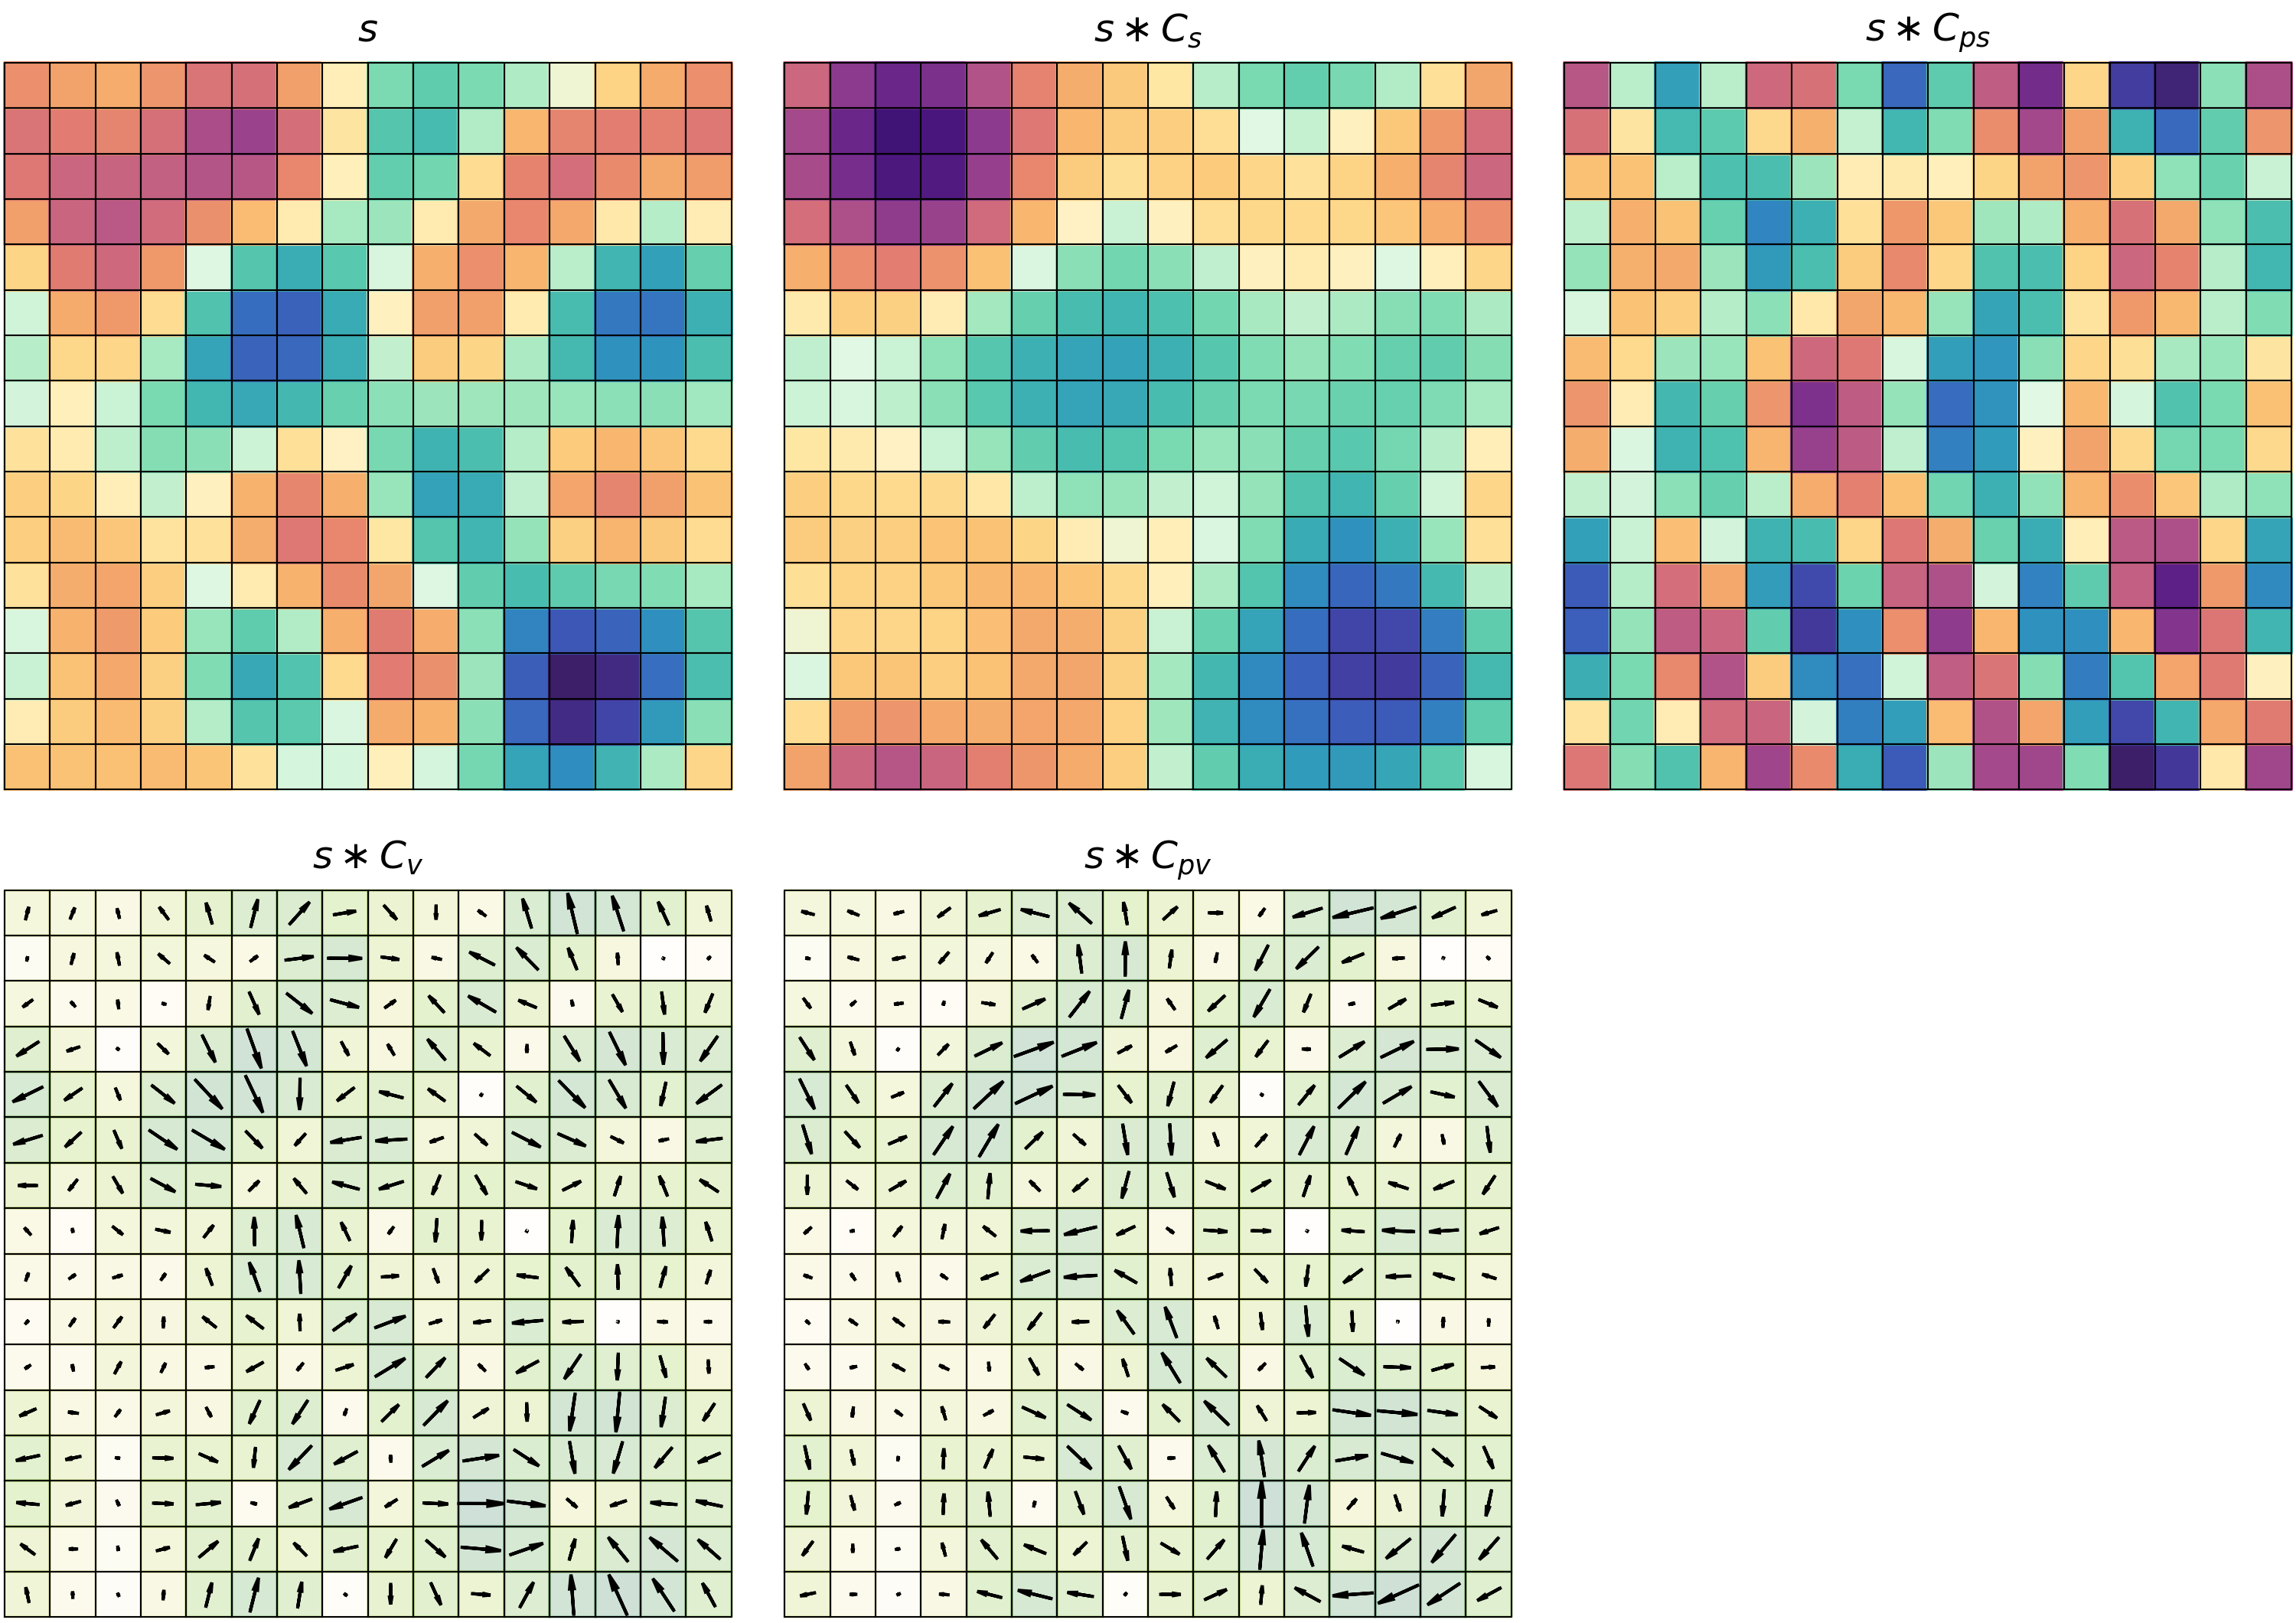
\includegraphics[width=\textwidth]{notebooks/monomials_1.png}
  \end{center}
  \caption{A scalar image $s$ and convolutions with four chosen filters.}
\end{hoggfigure}
Now show contractions of products of those images.
\begin{hoggfigure}
  \begin{center}
    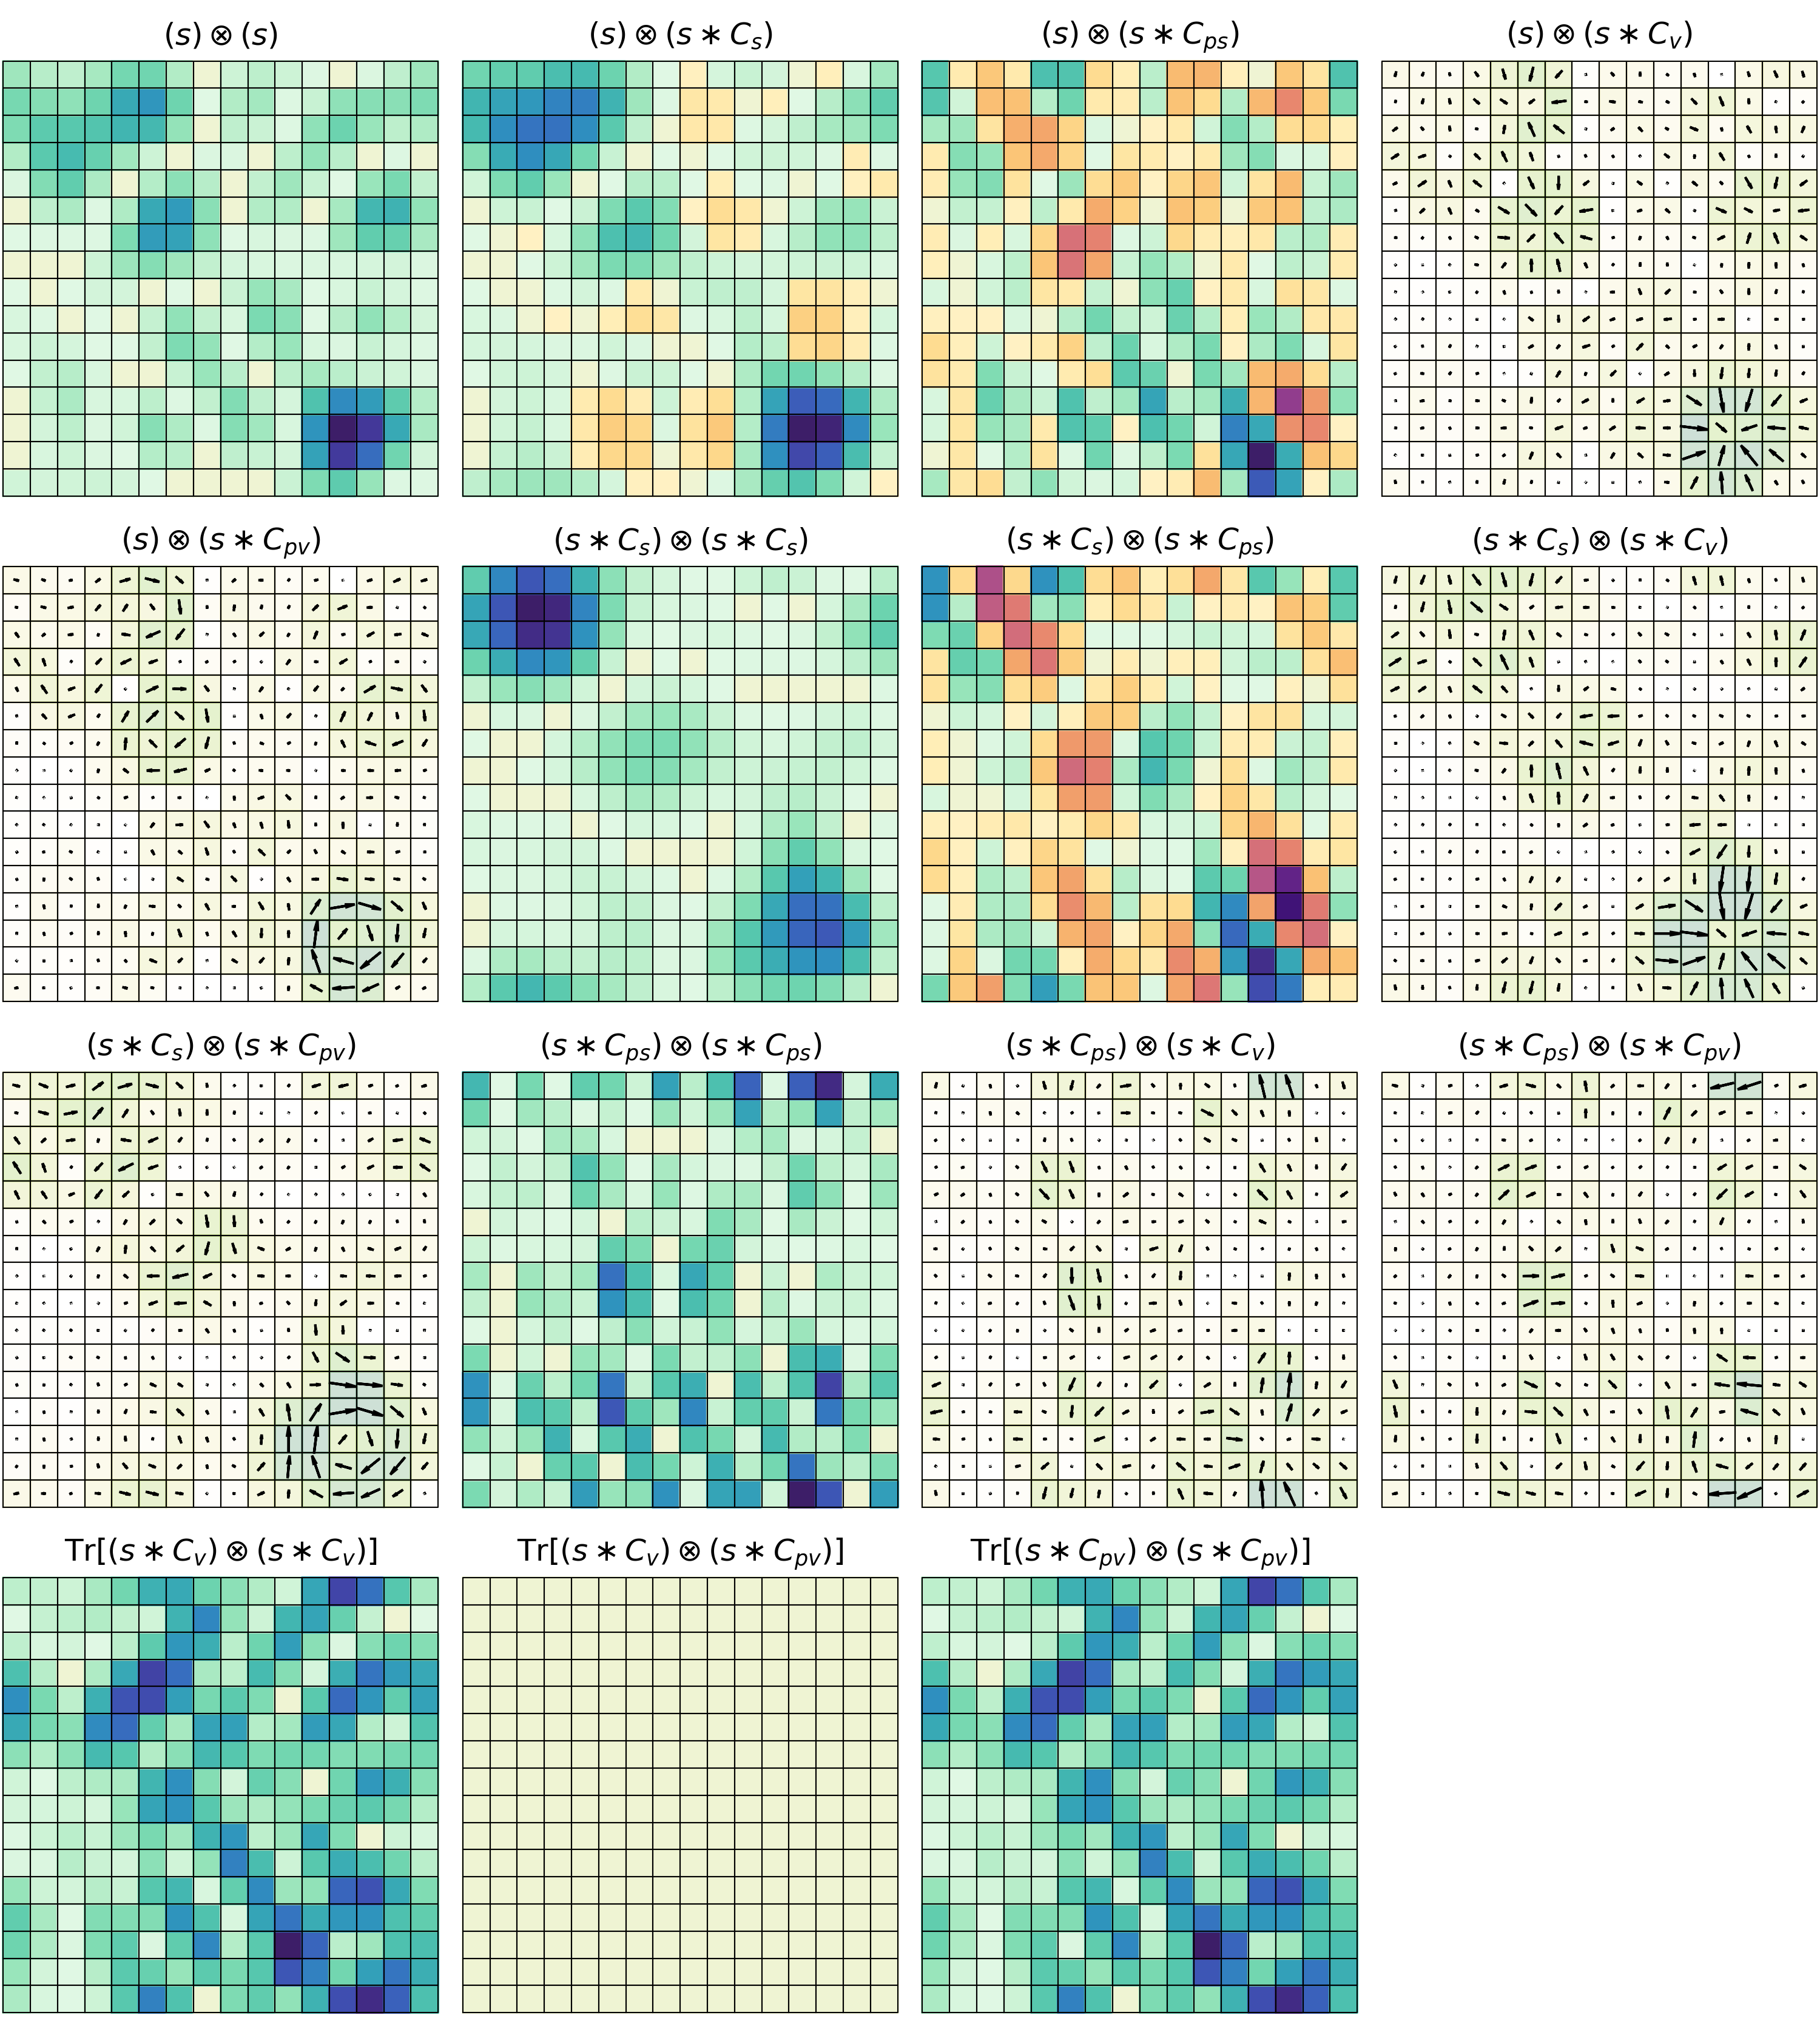
\includegraphics[width=\textwidth]{notebooks/monomials_2.png}
  \end{center}
  \caption{All unconvolved second-degree monomials of $s$, given four chosen filters. For the \tensor{2}{p} outputs (order $k=2$), we traced them back to scalars. HOGG ASKS: WHAT DOES THAT MEAN?}
\end{hoggfigure}
\end{comment}

We think of each building block of our architecture as a layer whose input and output is a set of images grouped by tensor order and parity. This is due to the key constraint that we can only add geometric images that share tensor order and parity. This partitioning also allows us to efficiently batch operations. The operation of each layer is either convolution, contraction, polynomial, or applying a nonlinear activation function.

A convolution layer takes a set of images and a set of convolution filters. For each filter, we take a weighted sum of the images of a particular tensor order and parity and apply the convolution\footnote{The geometric convolution package is implemented in JAX, which in turn uses TensorFlow XLA under the hood. This means that convolution is actually cross-correlation, in line with how the term in used in machine learning papers. For our purposes this results in at most a sign change, which will come out in the parameterization.} on that sum with that filter. Unlike a traditional CNN where the filters are parameterized, our filters are fixed to enforce the equivariance, and the weights of the weighted sums are the parameters. A convolution layer can also have an optional dilation where the filters are dilated before convolving. Dilations are helpful for expanding the effective size of the filters without having to calculate the invariant filters for larger $M$, which grows quickly; see \cite{convolution_math} for a description of dilated convolution. If we use filters with tensor order greater than 0, the tensor order of the images will continue to grow as we apply convolutions. Thus we need a way to reduce the tensor order -- we do this with the contraction layer.

Given an input layer and a desired tensor order, the contraction layer performs all unique contractions to get the layer to that tensor order. Each unique contraction thus results in a different image. We always end the neural network with a contraction layer to return the images to the proper tensor order. Since contractions can only reduce the tensor order by multiples of 2, the last convolution layer before the final contraction must result in images of order $k'' + 2N$ for some $N \in \mathbb{N}$ which may be different per image. We also may include contraction layers after each convolution to cap the tensor order of each layer to avoid running out of memory as the tensor order grows. In practice, $k=5$ seems to be a good max tensor order.

A polynomial layer takes a set of images and a polynomial degree and computes the full polynomial of all the images with each other using the tensor product of geoemtric images, up to the degree of the polynomial. Typically, this will result in a combinatorial blowup of images; we can take parameterized sums along the way to reduce the number of images created. We could also do a smaller set of products if we have some special domain knowledge. However, in practice it is usually better to use nonlinear activations functions, as in typically done in machine learning.

The final type of layer is a nonlinear activation layer. In order to maintain equivariance, we can either apply a nonlinearity to a scalar, or scale our tensors by a nonlinearity applied to the norm of the tensor CITE PAPER. For this paper, we used the first strategy. We apply all possible contractions to all even tensor order images to reduce them to scalars, apply the nonlinearity, then return those images to the layer. Any typical nonlinearity works -- ReLU, leaky ReLu, sigmoid, etc.

\subsection{Our Architectures}

\begin{comment}
There can also be pooling and unpooling layers.
There can even non-simply connected architectures, in which one path pools and unpools and the other path doesn't (as in map2map; CITE).

That is, there are myriad choices, for the investigator to choose through intuition or validation.
In addition there are choices about loss function, dropouts, and batch size, as in all machine-learning contexts.

Absent contractions, the tensor order will tend to grow as the number of layers increases.
We imagine that it will be useful or necessary to limit the maximum order $k$ of tensors in any channel at each layer.
This will require contractions to keep pace with convolutions and outer products to limit total tensor order.
\end{comment}

\section{Example Problems}\label{sec:examples}

The problem we are trying to solve is the following: Given a dynamical system such as a gif or a turbulent fluid simulation, can we predict the future steps of the system? Let $A_k$ be the geometric image at timepoint $k$ in the simulation. Given $A_k$, we want to predict $A_{k+1}$, although we will train our model to predict the difference $A_{k+1} - A_k$. Thus we are trying to learn the function $Net(A_k, \theta)$ parameterized by $\theta$ such that the loss between $A_{k+1}$ and $A_k + Net(A_k, \theta)$ is minimized. For our loss we will use the root mean squared error (RMSE). To improve training we will use the loss over two steps, so if $\widetilde{A}_{k+1} = A_k + Net(A_k, \theta)$ then
$$\text{Loss} = \text{RMSE}(A_{k+1}, \widetilde{A}_{k+1}) + \text{RMSE}(A_{k+2}, \widetilde{A}_{k+1} + Net(\widetilde{A}_{k+1}, \theta))$$

One key fact relevant to the construction of our neural network is that the input have the same tensor order. Thus as the tensor order of our images increases as we apply convolutions, we must perform an appropriate number of contractions at the end to bring them back down to the original size. We start by finding the invariant filters of even and odd parity of tensor order 1 and 2. We may omit the scalar filters because later we will perform all possible contractions, including the one on the two axes of of 2-0 tensors 0, 1, and 2 that revert them to the scalar filters. As we see in fig. \ref{fig:filters23}, this leaves us with 9 filters.

Next we have a sequence of convolutional layers, much as in a typical CNN. The first layer applies the 9 convolution filters to the input image. We take linear combinations of each output image and feed those sums each into the same 9 filters for a second layer. These linear combinations make the layers fully connected, with the caveat that we can only add geometric images if they have the same parity and tensor order. Next we have a quadratic layer where we take the outer product of every image output from the second layer.

Then we apply one final convolution to linear combinations of the quadratic layer. In this final layer, we only apply the convolution if the parity would match the input images parity, and the tensor order could be contracted down the the original images tensor order. For example, if the original image had order 1 and parity 0, then an image with tensor order 5 and parity 0 would only be convolved with 2-0 tensor filters. Finally, we apply all possible unique contractions to return the images to the original images tensor order, and we take the linear combination of all those resulting images. Parameters are used whenever we are taking linear combinations, so in the convolution layers and after doing the contractions.

\section{Related work}\label{sec:related}

The most common method to design equivariant maps is via group convolution, on the group or on the homogeneous space where the features lie. Regular convolution of a vector field $f: (\mathbb{Z} /N \mathbb{Z})^d \to \mathbb{R}^c$ and a filter $\phi: (\mathbb{Z} /N \mathbb{Z})^d \to \mathbb{R}^c$ is defined as
\begin{equation}\label{eq:1}
    f*\phi(x)= \sum_{y\in(\mathbb{Z} /N \mathbb{Z})^d} \underbrace{\langle f(y), \phi(y-x)\rangle}_{\text{scalar product of vectors}}=\sum_{y\in(\mathbb{Z} /N \mathbb{Z})^d} \sum_{j=1}^c \underbrace{f^j(y) \phi^j(y-x)}_{\in \mathbb{R}}
\end{equation}
Our generalization of convolution replaces this scalar product of vectors by the outer product of tensors. Probably the most related
work is by Brandstetter et al. \cite{ref1} who replace it by the geometric product of multivector inputs and multivector filters of a Clifford Algebra.

\subsection{Clifford Convolution}
This paper deals with multivector fields, i.e.: vector fields $f:\mathbb{Z}^2 \to (Cl_{p,q}(\mathbb{R}))^c$. The real Clifford Algebra $Cl_{p,q}(\mathbb{R})$ is an associative algebra generated by $p+q=d$ orthonormal basis elements: $e_1, \ldots, e_{p+q}\in \mathbb{R}^d$ with the relations:
\begin{eqnarray}
     e_i\otimes e_i = +1& (i\leq p),  \\
     e_j \otimes e_j = -1& (p<j\leq n),\\
     e_i \otimes e_j = -e_j \otimes e_i & (i\neq j).
\end{eqnarray}
For instance, $Cl_{2,0}(\mathbb{R})$ has the basis $\{1, e_1, e_2, e_1\otimes e_2\}$ and is isomorphic to the quaternions $\mathbb{H}$.

The Clifford convolution replaces the elementwise product of scalars of the usual convolution of \eqref{eq:1} by the geometric product of multivectors in the Clifford Algebra:
\begin{equation}
    f*\phi(x)= \sum_{y\in(\mathbb{Z} /N \mathbb{Z})^d} \sum_{j=1}^c \underbrace{f^j(y) \otimes \phi^j(y-x)}_{\in Cl_{p,q}(\mathbb{R})},
\end{equation}
where $f:\mathbb{Z}^2 \to (Cl_{p,q}(\mathbb{R}))^c$ and $\phi:\mathbb{Z}^2 \to (Cl_{p,q}(\mathbb{R}))^c$

The Clifford Algebra $Cl_{p,q}(\mathbb{R})$  is a quotient of the tensor algebra \begin{equation}
    T(\mathbb{R}^d)= \bigoplus_{k\geq 0} \underbrace{\mathbb{R}^d\otimes \ldots \otimes {\mathbb{R}^d}}_{k \text{ times}}= \bigoplus_{k\geq 0} (\mathbb{R}^d)^{\otimes k},
\end{equation} 
by the two-side ideal $\langle\{v\otimes v - Q(v): v \in \mathbb{R}^d\}\rangle$, where the quadratic form $Q$ is defined by $Q(e_i)=+1$,if  $i\leq p$, and $Q(e_j)=-1$, else $p<j\leq n$.
Our geometric images are functions $A:(\mathbb{Z}/N\mathbb{Z})^d \to \mathcal T_{d,k,p}$, where $\mathcal{T}_{d,k,p}= (\mathbb{R}^d)^{\otimes k}\subset T(\mathbb{R}^d)$. They can be related with the Clifford framework by seeing them as $N$-periodic functions from $\mathbb{Z}^d$ whose image is projected via the quotient map on the Clifford Algebra. This projection can be seen as a contraction of tensors. 

The Clifford convolution is not equivariant under multivector rotations or reflections. But the authors derive a constraint on the filters for $d=2$ which allows to build generalized Clifford convolutions which are equivariant with respect to rotations or reflections of the multivectors. That is, they prove equivariance of a Clifford layer under orthogonal transformations if the filters satisfies the constraint: $\phi^i (Rx) = R\phi^i(x)$.

Part of our work can be studied under the unified framework for group equivariant networks on homogeneous spaces derived from a Fourier perspective proposed in \cite{ref2}. 
\subsection{Unified Fourier Framework}
In \cite{ref2}, they consider general tensor-valued feature fields, before and after a convolution.  Their fields are functions $f : G/H \to V$ over the homogeneous space $G/H$ taking values in the vector space $V$ and their filters are kernels $\kappa: G \to Hom (V,V')$. Essentially, their convolution replaces the scalar product of vectors of traditional convolution by appliying an homomorphism. In particular, if $G$ is a finite group and $H=\{0\}$, they define convolution as
\begin{equation}
    \kappa* f(x)= \frac{1}{|G|}\sum_{y\in G}\underbrace{\kappa(x^{-1}y)f(y)}_{\in V'}.  
\end{equation}
They give a complete characterization of the space of kernels for equivariant convolutions. In our framework, the group is $\mathbb{Z}/N\mathbb{Z}$ and the kernel is an outer product by a filter $C$: $\kappa(g)A(g)=A(g)\otimes C(g)$. Note that $\mathbb{Z}/N\mathbb{Z}$ is neither an homogeneous space of $O(d)$ nor of $B^d$

We can analize our problem from an spectral perspective, in particular we can describe all linear equivariant using representation theory, using similar tools as in the proof of the ``only if'' part of Theorem 1 in \cite{ref3}. This theorem states that convolutional structure is a sufficient and a necessary condition for equivariance to the action of a compact group. Some useful references about group representation theory are \cite{ref5}, a classical book about the theory of abstract harmonic analysis and \cite{ref6}, about the particular applications of it.

\subsection{Linear equivariant maps}
In this work we define an action  over tensor images of $O(d)$, by rotation of tensors in each pixel; of $B^d$ by rotating the grid of pixels and each tensor in the pixel; and of $(\mathbb{Z}/N \mathbb{Z})^d$ by translation of the grid of pixels. The action of each one of these groups $G$ over $\mathcal{T}_{d,k,p}$
\begin{equation}
    \Phi_{d,k,p}: G \to GL_{con} (\mathcal{T}_{d,k,p}),
\end{equation}
can be decomposed into irreducible representations of $G$:
\begin{equation}
    \Phi_{d,k,p} \equiv \bigoplus_{\pi \in \hat{G}} m_{d,k,p}(\pi) \pi.
\end{equation}
That is, there is a basis of the Hilbert space $\mathcal{T}_{d,k,p}$ in which the action of $G$ is defined via a linear sparse map. In the case of $G$ finite, for all $g\in G$ there is a matrix $P$ splitting the representation in the Hilbert space into its irreducible components
\begin{equation}
    P^{-1} \Phi_{d,k,p}(g)P=\bigoplus_{\pi \in \hat{G}} m_{d,k,p}(\pi) \pi(g)
\end{equation}

Consider now linear maps between Tensor images:
\begin{equation}
    \mathcal{C}:\mathcal{T}_{d,k,p} \to \mathcal{T}_{d',k',p'}
\end{equation}
Linear equivariant maps satisfy that  $\mathcal{C}\circ \Phi_{d,k,p} = \Phi_{d',k',p'} \circ \mathcal{C}$. That is, if $\tilde{\mathcal{C}}$ is the representation of $\mathcal{C}$ in the above basis,
\begin{equation}
    \tilde{\mathcal{C}} \circ \bigoplus_{\pi \in G} m_{d,k,p}(\pi) \pi = \bigoplus_{\pi \in G} m_{d',k',p'}(\pi) \pi \circ \tilde{\mathcal{C}}.
\end{equation}
By Schur's Lemma, this implies that $\mathcal{C}\equiv \bigoplus_{\pi \in G} m_{d,k,p}(\pi) Id_{d_\pi}$.

The power of representation theory is not limited to compact groups. Mackey machinery allow us to study for instance semidirect products of compact groups and other groups, and in general to relate the representations of a normal subgroup with the ones of the hole group. This is the spirit of \cite{ref4}, which makes extensive use of the induced representation theory. An introduction to this topic can be found in Chapter 7 in \cite{ref5}.

\subsection{Steerable CNNs}
This paper deals exclusively with signals $f: \mathbb{Z}^2 \to \mathbb{R}^k$. They consider the action of \textit{p4m} on $\mathbb{Z}^2$ by translations, rotations by 90 degrees around any point, and reflections. This group is a semidirect product of $\mathbb{Z}^2$ and $H= D^4$ (also called $B^2$). Every $x\in \text{\textit{p4m}}$ can be written as $x=tr$, for $t\in \mathbb{Z}^2$ and $r\in D^4$. They show that equivariant maps with respect to representations $\rho$ and $\rho'$ of rotations and reflections $H$ lead to equivariant maps with respect to certain representations of $G$ $\pi$ and $\pi'$. This means that if we find a linear map $\phi: f \mapsto \phi f$ such that $\phi \rho(h)f=\rho'(h)\phi f$ for all $h\in H$, then for the representation of $G$ $\pi'$ defined by
\begin{equation}\label{eq:2}
    \pi'(tr)f(y) = \rho(r) [f ((tr)^{-1}y)], \quad tr\in G, y \in \mathbb{Z}^2,
\end{equation}
we automatically have that $\phi \pi(g)f=\pi'(g)\phi f$ for all $g\in G$. This is the representation of $G$ induced by the representation $\rho$ of $H$

Note that, the similarity between the definition of the action of $B^d$ on tensor images and equation \eqref{eq:2}. The convolution with a symmetric filter produces easily an equivariant map with respect to  the action of the semidirect product of $\mathbb{Z}^d$ and $B^d$ on the tensor images. 

\section{Overview of the study of equivariant maps for machine learning}
Restricting the learning to a hypothesis class where all the functions are equivariant with respect to some group action is a is a powerful tool widely used in machine learning.

\subsection{Motivation}\label{sec:related2}
It is believed that engineering a model to be equivariant improves its generalisation and accuracy.  The generalisation benefit of equivariant linear models has been quantified in \cite{elesedy2021provably}, and the  benefit of incorporating invariance in kernel ridge regression when the target is invariant to the action of a compact group has been quantified in \cite{elesedy2021kernel}. This benefit has been observed in many applications, for instance \cite{wang2021incorporating}. Also, it is believed to be a powerful remedy against the lack of data and an alternative to data augmentation, a technique to train models that preserve symmetries by adding samples to the training set which are transformed versions of other samples. For instance, \cite{wang2022data} derives generalization bounds for data augmentation and for equivariant networks, in the setting of dynamics forecasting of non-stationary and
non-mixing time series.

Other reason is that constraining linear layers in neural networks to be equivariant allows, in certain cases, to approximate any continuous invariant function. For example, in \cite{yarotsky2018universal} they show that invariant networks with respect to a subgroup of the symmetric group can universally approximate any real-valued continue function from $\mathbb{R}^n$; and in \cite{dym2020universality}, a similar result is proved for functions from point clouds to some representation of $SO(3)$. \cite{bokman2022zz} deals too with point clouds. Kumagai et al. proposed in \cite{kumagai2020universal} a unified method to obtain universal approximation theorems for equivariant maps by CNNs. Note that our convolution is a particular case of the general group convolution that they study. They consider a group $G$ that acts on sets $\mathcal{S}$ and $\mathcal{T}$, a $G$-invariant measure $\nu$ on $\mathcal{S}$, a $G$-invariant functions $v: \mathcal{S} \times \mathcal{T} \rightarrow \mathbb{R}$ and $b \in \mathcal{C}(\mathcal{T})$. They define the biased $G$-convolution $C_{\nu, v, b}: \mathcal{C}(\mathcal{S}) \rightarrow \mathcal{C}(\mathcal{T})$ as
\begin{equation}
C_{\nu, v, b}[x](t):=\int_{\mathcal{S}} v(t, s) x(s) d \nu(s)+b(t)
\end{equation}
Thus our maps can be used to approximate continuous non-linear equivariant maps.

The interest in equivariant maps for machine learning has lead to a huge garden of methods for various kinds of data and to the reinvention of the same algorithms in different application domains. Also there are some works about the unifying principles. 

Irreducible representations or invariant theory are typically
used to parameterize the space of equivariant functions. 

\subsection{Representation theory}
The first work using representation theory for invariant and equivariant neural networks was the paper of  Wood et al. \cite{WOOD199633} from 1996. More recent incarnations of these ideas include the works of \cite{makadia}, \cite{ref4}, \cite{Cohen16}, \cite{cohen2019gauge}, \cite{de2020gauge} and \cite{esteves}.

\subsection{Invariant theory}
One can use classical invariant theory to compute the generators of the algebra of invariant polynomials. For instance, in \cite{2022blum-smith-villar-equivariant} we show how to use the generators of the algebra of invariant polynomials to produce a parameterization of equivariant functions for certain groups and actions. A classical introduction to the topic can be found in \cite{weyl}. This approach is inspired by the he physical sciences, where the data is subject to rules coming from coordinate freedoms and conservation laws. In previous work \cite{villar2021scalars, villar2022dimensionless, yao2021simple} we used these geometric rules to develop modified machine-learning methods that are restricted to exactly obey group-theoretic equivariances in physics contexts. The same idea has explored in \cite{haddadin2021invariant}, \cite{Gripaios_2021}, \cite{yao2021simple}.

\subsection{Graph Neural Networks}
Graph neural networks (GNNs) can also be seen as equivariant functions that take a graph (or an hypergraph) $A\in (\mathbb{R}^n)^{\otimes k}$ and output an embedding $f(A)\in (\mathbb{R}^n)^{\otimes k'}$ so that $f(\Pi *A)=\Pi*f(A)$, for any relabeling of the vertexes induced by a permutation $\Pi$. In \cite{maron2018invariant}, they give a characterization of all permutation invariant and equivariant linear layers. Graph methods are versatile, for instance, a common approach to define convolutions on meshes is to interpret them as a graph and apply graph convolutional networks \cite{de2020gauge}. There are many works about the universal approximation properties of permutation-invariant functions by certain classes of GNNs (see, for instance \cite{kumagai2020universal}), but also, about the limitation of the expresive powers of GNNs via graph isomorphism tests (see \cite{power}). These two perspectives are not only connected but also, they are equivalent, as shown in \cite{graphisotest}.

\section{Discussion}\label{sec:discussion}

One of the strange aspects of this work is that there are two groups acting.
One is a continuous group (the Euclidean group) of translations and rotations (and reflections).
This group motivates the index summation rules and the other geometric operations in the functions we construct.
The other group is a discrete group $G_{N,d}$ appropriate for $d$-cube lattices of points; it is a sub-group of the continuous group.
This is the group we use to average the filters (to make invariant filters) and we use to define equivariance for functions of geometric images.
There are other possible image representations---other than values in pixels---that might create more continuous concepts of images.
For example, if the data are on the surface of the sphere (the sky, perhaps), it could be represented with tensor spherical harmonics, and be subject to transformations by a continuous rotation group.

But if we think in terms of a physical, generative model for imaging: Usually an image is ``taken'' of a continuous world.
That is, the kinds of geometric images we consider in this work would mainly be discretized views or samples of a larger, continuous world.
That world is subject to transformations by continuous symmetries, maybe even gauge symmetries.
It remains an open question how to think about how to use the operations and symmetries of these large, continuous groups that govern the world being viewed, when the data are only discrete, finite views of that world.

HOGG: It is interesting that the convolution operations look (in many cases) very much like discrete versions of vector calculus operations, like div, grad, curl, and so on.
(Refer back to particular panels of particular figures.)
That's interesting, and potentially useful.

Note that we never take eigenvalues. But these are also real scalars in some cases.

Note that \tensor{k}{-} (pseudo) filters only exist for certain triples of $(d, m, k)$.

We could have added the determinant operation and eigenvalues.....

\paragraph{Acknowlegements:}
It is a pleasure to thank
Leslie Greengard (Flatiron),
Teresa Huang (JHU),
Kate Storey-Fisher (NYU),
Kaze Wong (Flatiron),
and the Astronomical Data Group at the Flatiron Institute for valuable discussions and input.
This project made use of Python~3 \cite{python3}, numpy \cite{numpy}, matplotlib \cite{matplotlib}, and cmastro \cite{cmastro}.
All code used for making the data and figures in this paper are available at \url{https://github.com/davidwhogg/GeometricConvolutions}.

\bibliographystyle{plain}
\raggedright
\bibliography{ref}
\end{document}









%SOLEDAD:
Now imagine that we want to find \emph{all} linear equivariant functions that go from an input $k$-$p$-tensor image of side length $N$ to an output $k'$-$p'$-tensor image of side length $N'$ (where either $N$ is divisible by $N'$, or $N'$ is divisible by $N$).
Here are the linear operations (linear in the input image) that are permitted:
\begin{enumerate}
    \item Perform a convolution and index contraction. For this step there are two qualitatively different options:
        \begin{itemize}
            \item Choose an integer $\ell$ in the range $0\leq\ell\leq k$ such that $(k'-k+2\,\ell)>0$.
              Convolve the input $k$-tensor image with a $(k'-k+2\,\ell)$-tensor invariant filter of parity $p\,p'$.
              Contract the resulting $(k'+2\,\ell)$-tensor image (of parity $p'$) with the Kronecker delta $\ell$ times, always choosing at least one index from the indices of the input image.
              %There are $$\frac{1}{\ell!}\,\prod_{i=1}^{\ell}\left[\choose{k'+2\,i}{2}-\choose{k'-k+2\,i}{2}\right]$$ possible choices for these $\ell$ Kronecker contractions.
            \item Choose an integer $\ell$ in the range $0\leq\ell\leq k-d+1$ such that $(k'-k+d-2+2\,\ell)>0$.
              Convolve the input $k$-tensor image with a $(k'-k+d-2+2\,\ell)$-tensor invariant filter of parity $-p\,p'$.
              Contract the resulting $(k'+d-2+2\,\ell)$-tensor image (of parity $-p'$) with the Levi--Civita symbol.
              %There are $$(d-1)!\,\left[\choose{k'+d-2+2\,\ell}{d-1}-\choose{k'-k+d-2+2\,\ell}{d-1}\right]$$ choices for this Levi--Civita contraction.
              Then contract the resulting $(k'+2\,\ell)$-tensor image (of parity $p'$) with the Kronecker delta $\ell$ times, always choosing one index from the indices of either the input image or of the Levi--Civita symbol.
              %There are $$\frac{1}{\ell!}\,\prod_{i=1}^{\ell}\left[\choose{k'+2\,i}{2}-\choose{k'-k+2\,i}{2}\right]$$ possible choices for these $\ell$ Kronecker contractions.
        \end{itemize}
    \item Perform (generally after the convolution and contraction) any index permutation you like (provided that $k'>1$).
      There are $k'!$ choices for the index permutation.
    \item Perform (generally after all the above) a pooling or unpooling step to get the image to side length $N'$.
\end{enumerate}
The objects obtained by this algorithm may not be linearly independent.

In principle there could also have been an \emph{eigenvalues} operator that is linear in the input and produces $d$ $0$-$p$-tensors.
But since any such operation can only reasonably be applied to $2$-$p$-tensors, and even for those, only Hermitian ones, we don't include this operation here.